\lstinputlisting[language=bash,basicstyle=\small]{python_codes/fieldstone_39/keywords}

\begin{center}
Code at \url{https://github.com/cedrict/fieldstone/tree/master/python_codes/fieldstone_39}
\end{center}

\par\noindent\rule{\textwidth}{0.4pt}
%%%%%%%%%%%%%%%%%%%%%%%%%%%%%%%%%%%%%%%%%%%%%%%%%%%%%%%%%%%%%%%%%%%%%%%%%%%%%%%%%%%%%%%%%%%%%

Before we dive in the implementation and the benchmarks, a side note which explains Eq.(3) 
of 
Choi \& Petersen \cite{chpe15}.
The Drucker-Prager yield function is given by the function $f$:
\[
{\cal F} = p \sin\phi + c\cos \phi - \tau_e
\]
where $\tau_e$ is the square root of the second invariant of the deviatoric stress
(the 'effective' deviatoric stress).
We have
\[
p=\frac{1}{2}(\sigma_1+\sigma_3) 
\]
and 
\[
\tau = \frac{1}{2}(\sigma_1-\sigma_3)
\]
Inserting these into ${\cal F}$ yields:
\[
{\cal F}= \frac{1}{2}(\sigma_1+\sigma_3) \sin\phi + c \cos\phi - \frac{1}{2}(\sigma_1-\sigma_3)
\]
The yield condition ${\cal F}=0$ can be reworked as follows:
\[
\sigma_1 - \frac{1 + \sin\phi}{1-\sin\phi} \sigma_3 - 2 \frac{\cos \phi}{1-\sin\phi} c = 0
\]
The third term can further be modified as follows:
\[
\frac{\cos \phi}{1-\sin\phi}
=\frac{\sqrt{1-\sin^2 \phi}}{\sqrt{(1-\sin\phi)^2}}
=\frac{\sqrt{(1-\sin \phi)(1+\sin\phi)}}{\sqrt{(1-\sin\phi)^2}}
=\sqrt{
\frac{1+\sin\phi}{1-\sin\phi}
}
\]
Finally, we define $N_\phi$ as follows 
\[
N_\phi=\frac{1+\sin \phi}{1-\sin\phi}
\]
so that the yield condition becomes:
\[
\sigma_1 - N_\phi \sigma_3 - 2 \sqrt{N_\phi} c = 0
\]
which is Eq.~3 of the article by Choi \& Petersen \cite{chpe15}.

\vspace{1cm}

Choi \& Petersen offer a solution to the problem of the angle of shear bands in 
geodynamic models. The underlying idea is based on simple modifications 
brought to existing incompressible flow codes. Note that the codes
featured in that paper also implemented elastic behaviour but this can 
be easily switched off by setting $Z=1$ in their equations.

Their plasticity implementation starts with a modification of the 
continuity equation:
\[
\vec\nabla\cdot\vec\upnu = R = 2 \sin\psi \, \dot{\varepsilon}_p
\]
where $R$ is the dilation rate, $\Psi$ is the dilation angle 
and $\dot{\varepsilon}_p$ is the square root of 
the second invariant of the plastic strain rate.

Under this assumption, the deviatoric strain rate tensor is given by
\begin{equation}
\dot{\bm \varepsilon}^d(\vec\upnu)
= \dot{\bm \varepsilon}(\vec\upnu)- \frac{1}{3} Tr[\dot{\bm \varepsilon}(\vec\upnu)] {\bm 1}
= \dot{\bm \varepsilon}(\vec\upnu)- \frac{1}{3} \vec\nabla\cdot\vec\upnu \; {\bm 1}
= \dot{\bm \varepsilon}(\vec\upnu)- \frac{1}{3} R \; {\bm 1}
\end{equation}
Turning now to the momentum conservation equation:
\begin{eqnarray}
-\vec\nabla p + \vec\nabla \cdot {\bm \tau} 
&=& -\vec\nabla p + \vec\nabla \cdot (2 \eta \dot{\bm \varepsilon}^d(\vec\upnu)) \nonumber \\
&=& -\vec\nabla p + \vec\nabla \cdot \left[ 2 \eta \left(\dot{\bm \varepsilon}(\vec\upnu)- \frac{1}{3} R \; {\bm 1}\right) \right] \nonumber\\
&=& -\vec\nabla p 
+ \vec\nabla \cdot \left( 2 \eta \dot{\bm \varepsilon}(\vec\upnu)\right) -\frac{2}{3} \vec\nabla(\eta R) 
\label{chpeform}
\end{eqnarray}
The last term is then an addition to the right hand side of the momentum equation 
and its weak form is as follows:
\begin{equation}
\vec f' 
= \int_\Omega N_v \frac{2}{3} \vec\nabla(\eta R) dV
= \frac{4}{3} \sin \Psi \int_\Omega N_v \vec\nabla(\eta \dot{\bm \varepsilon}_p) dV
\end{equation}
This formulation proves to be problematic since in order to compute the gradient, we would
need the viscosity and the plastic strain rate on the mesh nodes and both these quantities
are effectively computed on the quadrature points. One option could be to project those quadrature
values onto the nodes, which may introduce interpolation errors/artefacts and/or smoothing. 
Another option is to resort to integration by parts:
\begin{equation}
\int_\Omega N_v \vec\nabla(\eta \dot{\bm \varepsilon}_p) dV
= \left[ N_v \eta \dot{\bm \varepsilon}_p \right]_\Gamma 
-\int_\Omega \vec\nabla N_v (\eta \dot{\bm \varepsilon}_p) dV
\end{equation}
The last term is now trivial to compute since the shape function derivatives, the viscosity
and the plastic strain rate are known at the quadrature points. Remains the surface term. 
We will neglect it for now to simplify our implementation and note that a) it will not directly 
affect what happens inside the domain, b) it could be somewhat important when shear bands
intersect with the free surface. Then 
\begin{equation}
\vec f' 
=
-\frac{4}{3}\sin\psi\int_\Omega \vec\nabla N_v (\eta \dot{\varepsilon}_p) dV
=
-\frac{2}{3} \int_\Omega \vec\nabla N_v (\eta R) dV
\end{equation}

Although the authors do indicate that they add a term in each rhs, it is not very clear how they deal with
the implementation issue above. We then propose an alternative: instead of explicitely removing the deviatoric 
part of the strain rate as in \eqref{chpeform} and replace the trace of the tensor by $R$, one could 
leave the term inside the matrix, thereby using a compressible form of the viscous block of the Stokes 
matrix. We will recover the same converged solution as before, but the path to convergence will be 
different that the first approach.
In what follows, we denote the original approach by Choi \& Petersen 'method 1' and the latter 'method 2'.
The ${\bm C}$ matrix is then 
\[
{\bm C}_{method\; 1}
=
\left(
\begin{array}{ccc}
2 &0 &0 \\
0 &2 &0 \\
0 &0 &1
\end{array}
\right)
\qquad\qquad
{\bm C}_{method\; 2}
=
\left(
\begin{array}{ccc}
4/3 &-2/3 &0 \\
-2/3 & 4/3 &0 \\
0 &0 &1
\end{array}
\right)
\]


Finally, we need to define what the plastic strain rate tensor is. When using a rigid plastic 
rheology, the only deformation mechanism {\it is} plasticity so that the plastic strain rate {\it is}
the strain rate. When using a visco-plastic rheology, the plastic strain rate is the strain rate 
of the zones above/at yield (the shear bands, where the vrm is active). REPHRASE

\begin{remark}
The rhs of the continuity equation is formulated as a function of the (effective) plastic strain rate so that 
in the case of multiple deformation mechanisms one should be careful about this term.
\end{remark}

\newpage 
%..........................................................
\subsection*{Benchmark \#1 - The simple brick}

%The setup is {\sl similar} to the one in Kaus (2010) \cite{kaus10}, the main difference being that 
%there is no weak inclusion at the bottom of the domain. 
The 2D Cartesian domain filled with a 
single rigid-plastic material characterised by a cohesion $c=10\text{MPa}$, an 
angle of friction $\phi$, a dilation angle $\psi$ and a density $\rho=2800\text{kg/m}^3$.
Gravity is set to $|g_y|=10\si{\metre\per\square\second}$.

\begin{center}
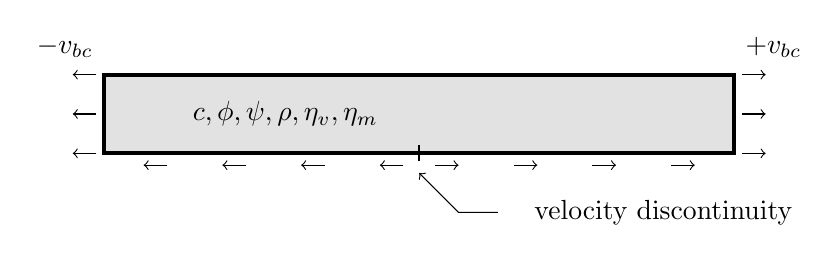
\begin{tikzpicture}
%\draw[fill=gray!23,gray!23](0,0) rectangle (10,3);
%\draw[step=0.5cm,gray,very thin] (0,0) grid (10,3); %background grid

\draw[fill=gray!23,gray!23](1,1) rectangle (9,2);

\draw[line width=0.5mm] (1,1)--(9,1)--(9,2)--(1,2)--cycle ;   

\draw[line width=0.3mm] (5,0.9)--(5,1.1); 

%left arrows
\draw [->] (0.9,1) -- (0.6,1);
\draw [->] (0.9,1.5) -- (0.6,1.5);
\draw [->] (0.9,2) -- (0.6,2);

\draw [->] (4.8,0.85) -- (4.5,0.85);
\draw [->] (3.8,0.85) -- (3.5,0.85);
\draw [->] (2.8,0.85) -- (2.5,0.85);
\draw [->] (1.8,0.85) -- (1.5,0.85);

%right arrows
\draw [->] (9.1,1) -- (9.4,1);
\draw [->] (9.1,1.5) -- (9.4,1.5);
\draw [->] (9.1,2) -- (9.4,2);

\draw [->] (5.2,0.85) -- (5.5,0.85);
\draw [->] (6.2,0.85) -- (6.5,0.85);
\draw [->] (7.2,0.85) -- (7.5,0.85);
\draw [->] (8.2,0.85) -- (8.5,0.85);

\node[] at (0.5,2.35) {$-v_{bc}$};
\node[] at (9.5,2.35) {$+v_{bc}$};

\node[] at (3.3,1.5) {$c,\phi,\psi,\rho,\eta_v,\eta_m$};
  
\draw [->] (6,0.25) -- (5.5,0.25) -- (5,0.75);
\node[] at (8.1,0.25) {velocity discontinuity};

\end{tikzpicture}
\end{center}


Extensional boundary conditions are as follows: 
\begin{itemize}
\item left boundary: $u=- \upnu_{bc}$, $v$ free;
\item right boundary: $u=+ \upnu_{bc}$, $v$ free; 
\item bottom boundary: $v=0$, $u=- \upnu_{bc}$ for $x<L_x/2$,  $u=+ \upnu_{bc}$ for $x>L_x/2$, and $u=0$ if $x=L_x/2$;
\item top boundary: zero traction.
\end{itemize}
For compressional boundary conditions the signs of all horizontal velocities should be reversed.
The nonlinear tolerance is set to $\text{tol}=10^{-6}$. Nonlinear iterations stop when 
maximum of the normalised nonlinear residual reaches the desired tolerance.
$\upnu_{bc}$ is chosen so that the background strain rate is $\dot\varepsilon_{bckgr}=10^{-15}\si{\per\second}$, 
i.e. $\upnu_{bc}=\dot\varepsilon_{bckgr} L_x/2$.

Following Choi \& Petersen \cite{chpe15}, we run the experiment with an associative ($\phi=\psi$) plasticity
and a non associative one ($\psi=0$, i.e. $R=0$). This second approach is essentially what many codes do (
i.e. $\vec\nabla\cdot\vec\upnu = 0$). We can also run the model with $\phi=\psi=0\si{\degree}$ so that 
we recover the von Mises plasticity yield criterion which is independent of pressure.  

The velocity, pressure, strain rate, dilation rate, and velocity divergence are shown hereunder both in 
extension and compression. Note that the domain has been substantially extended in the horizontal 
direction because of the wide shear band angles obtained in compression. It is now 80\si{\km} long 
and 10\si{\km} high (aspect ratio 8:1). 

Three angles are mechanically stable (e.g. \cite{kaus10}):
\[
\theta=\frac{\pi}{4}\pm \frac{\psi}{2} \qquad \text{Roscoe angle}
\]
\[
\theta=\frac{\pi}{4}\pm \frac{\phi}{2} \qquad \text{Coulomb angle}
\]
\[
\theta=\frac{\pi}{4}\pm \frac{\phi+\phi}{4} \qquad \text{Arthur angle}
\]
In the case of associative plasticity, $\phi=\psi$, so that all three angles are the same. 
Per row of elements, nodes or quadrature points, and per half of the domain (left and right) we find the location
with the highest strain-rate and record their coordinates.


\newpage
{\bf Extension}

\begin{center}
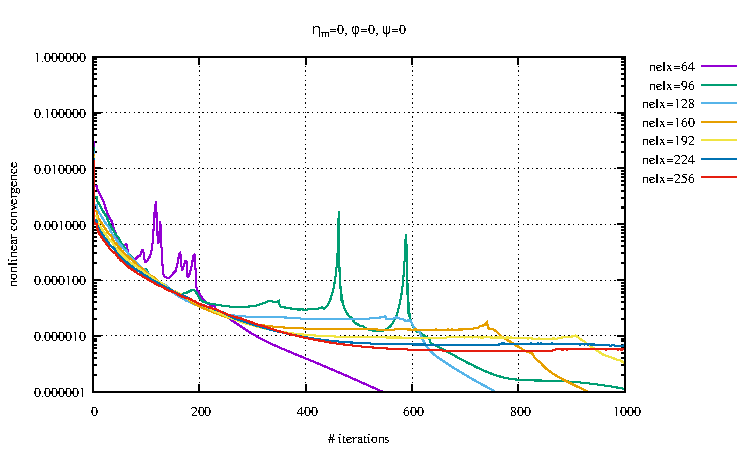
\includegraphics[width=.3\linewidth]{python_codes/fieldstone_39/benchmark1/extension/conv_phi0_psi0_etam0.pdf}
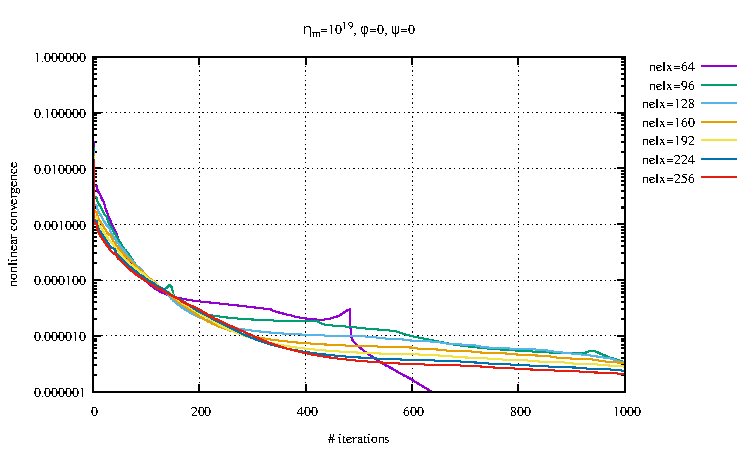
\includegraphics[width=.3\linewidth]{python_codes/fieldstone_39/benchmark1/extension/conv_phi0_psi0_etam19.pdf}
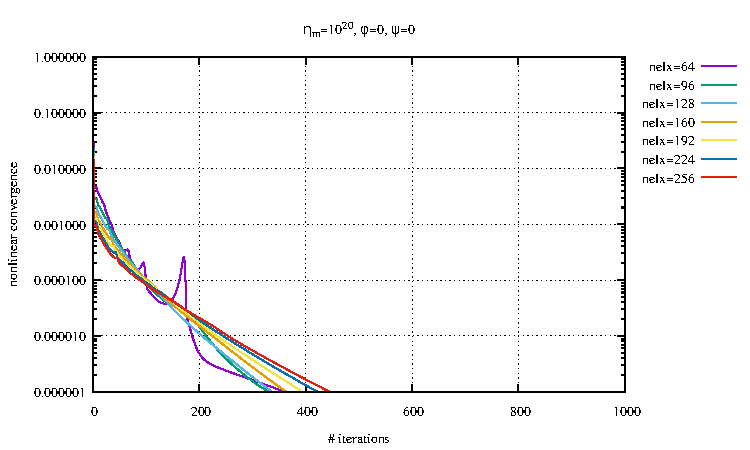
\includegraphics[width=.3\linewidth]{python_codes/fieldstone_39/benchmark1/extension/conv_phi0_psi0_etam20.pdf}\\
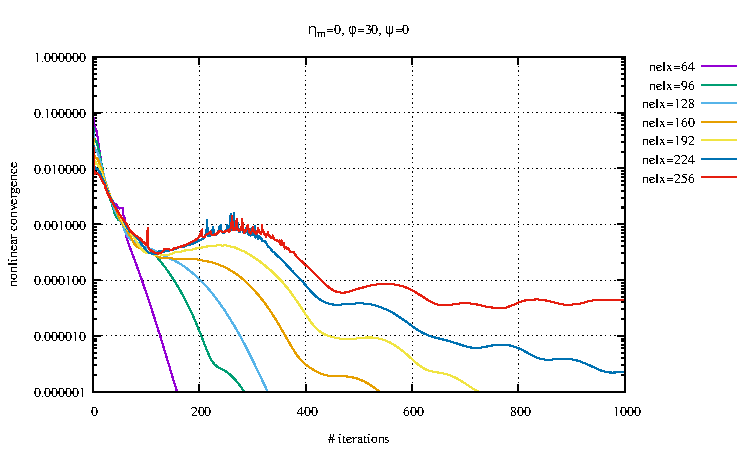
\includegraphics[width=.3\linewidth]{python_codes/fieldstone_39/benchmark1/extension/conv_phi30_psi0_etam0.pdf}
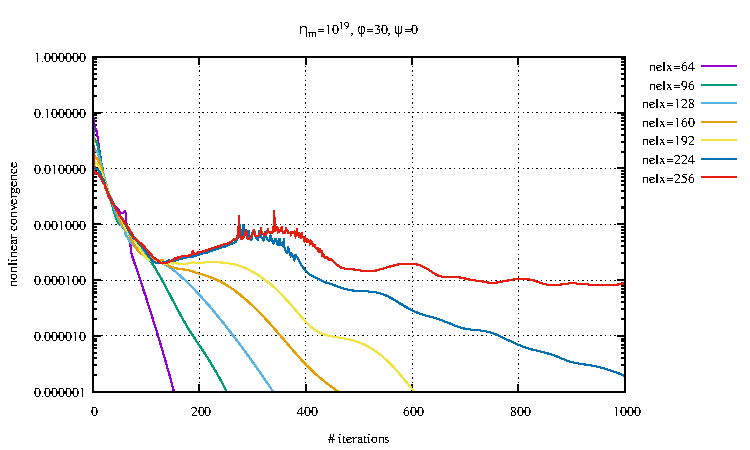
\includegraphics[width=.3\linewidth]{python_codes/fieldstone_39/benchmark1/extension/conv_phi30_psi0_etam19.pdf}
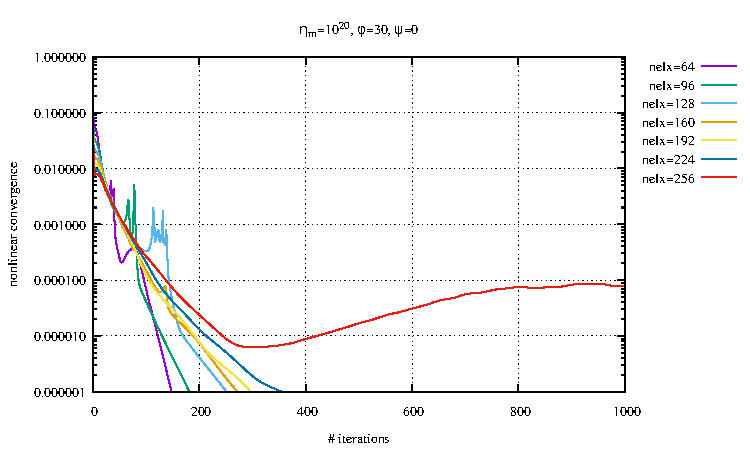
\includegraphics[width=.3\linewidth]{python_codes/fieldstone_39/benchmark1/extension/conv_phi30_psi0_etam20.pdf}\\
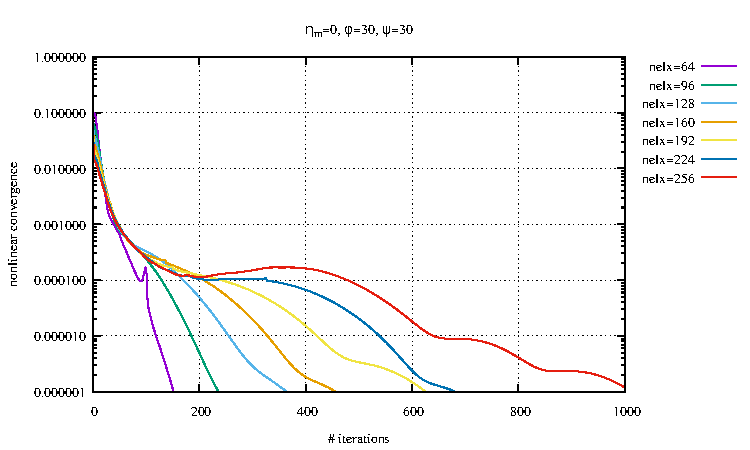
\includegraphics[width=.3\linewidth]{python_codes/fieldstone_39/benchmark1/extension/conv_phi30_psi30_etam0.pdf}
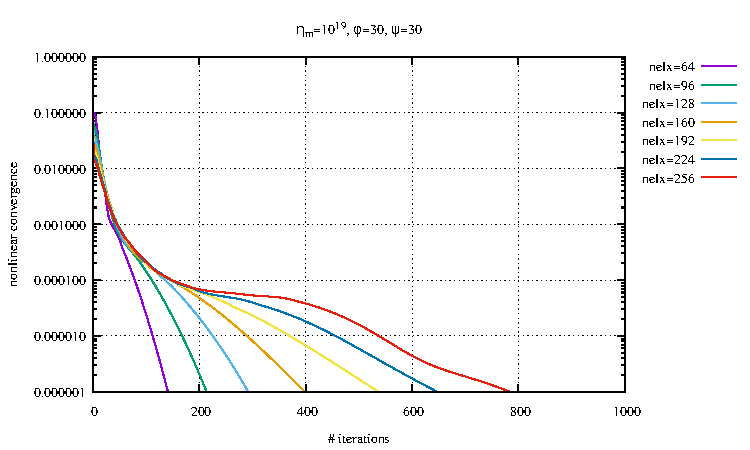
\includegraphics[width=.3\linewidth]{python_codes/fieldstone_39/benchmark1/extension/conv_phi30_psi30_etam19.pdf}
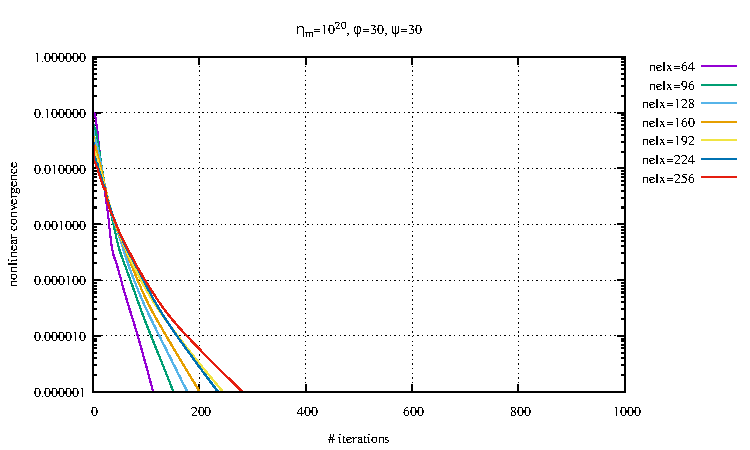
\includegraphics[width=.3\linewidth]{python_codes/fieldstone_39/benchmark1/extension/conv_phi30_psi30_etam20.pdf}\\
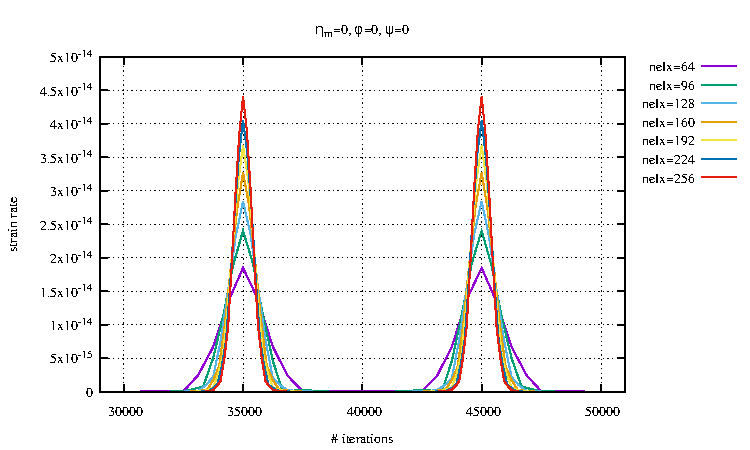
\includegraphics[width=.3\linewidth]{python_codes/fieldstone_39/benchmark1/extension/line_sr_phi0_psi0_etam0.pdf}
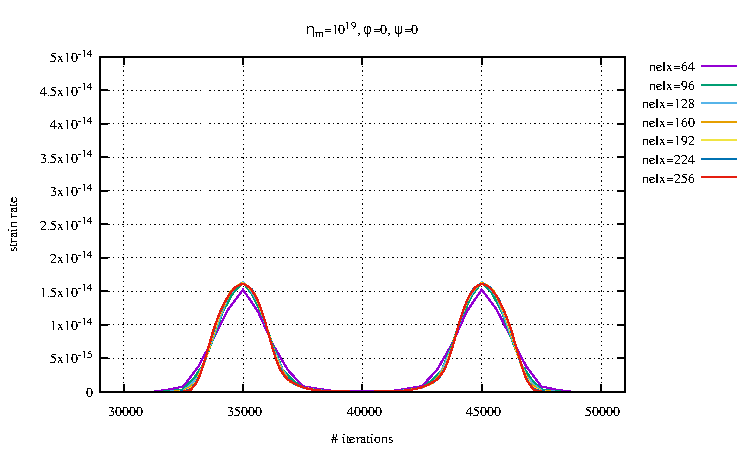
\includegraphics[width=.3\linewidth]{python_codes/fieldstone_39/benchmark1/extension/line_sr_phi0_psi0_etam19.pdf}
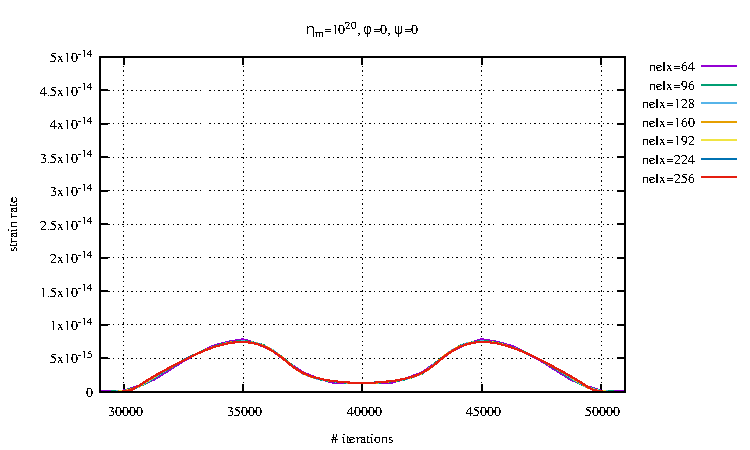
\includegraphics[width=.3\linewidth]{python_codes/fieldstone_39/benchmark1/extension/line_sr_phi0_psi0_etam20.pdf}\\
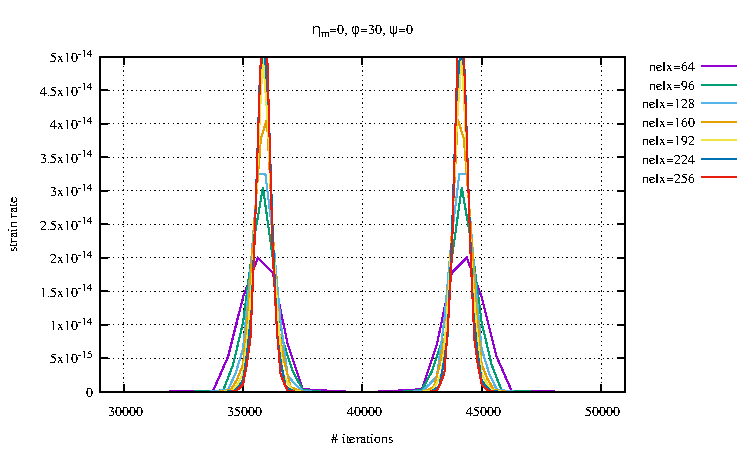
\includegraphics[width=.3\linewidth]{python_codes/fieldstone_39/benchmark1/extension/line_sr_phi30_psi0_etam0.pdf}
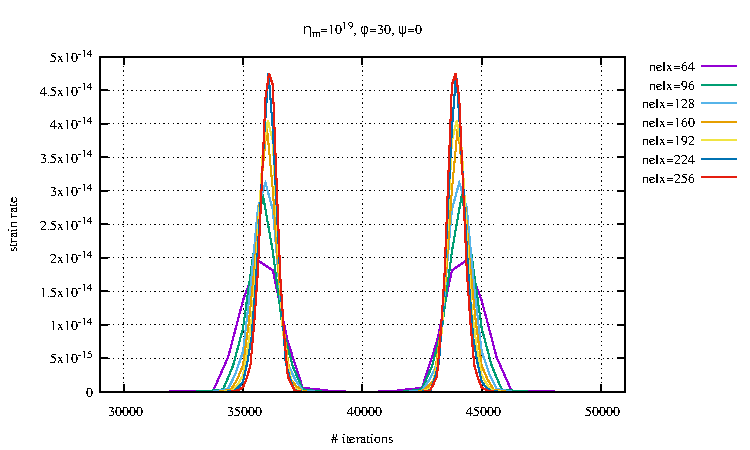
\includegraphics[width=.3\linewidth]{python_codes/fieldstone_39/benchmark1/extension/line_sr_phi30_psi0_etam19.pdf}
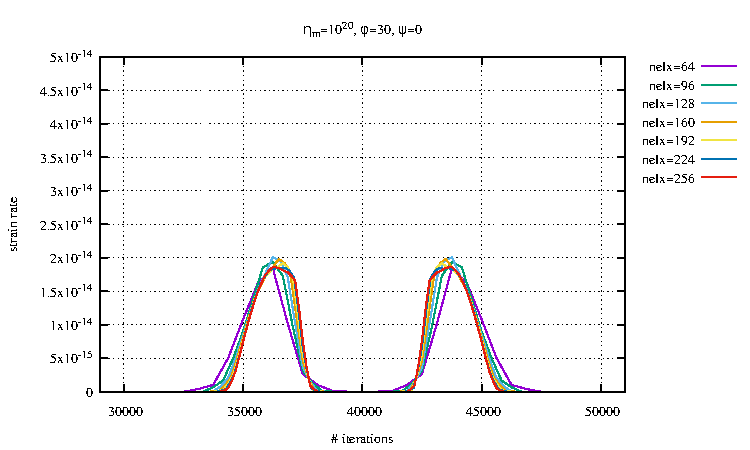
\includegraphics[width=.3\linewidth]{python_codes/fieldstone_39/benchmark1/extension/line_sr_phi30_psi0_etam20.pdf}\\
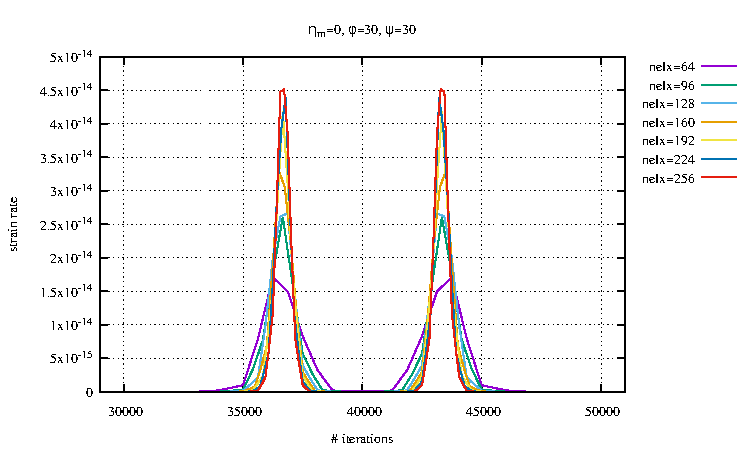
\includegraphics[width=.3\linewidth]{python_codes/fieldstone_39/benchmark1/extension/line_sr_phi30_psi30_etam0.pdf}
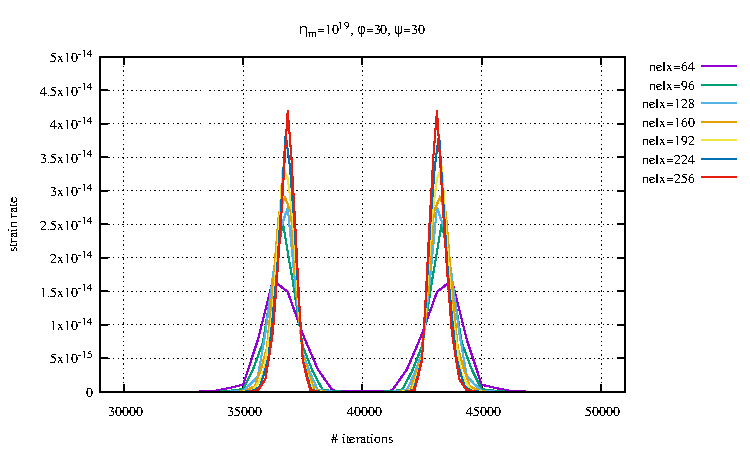
\includegraphics[width=.3\linewidth]{python_codes/fieldstone_39/benchmark1/extension/line_sr_phi30_psi30_etam19.pdf}
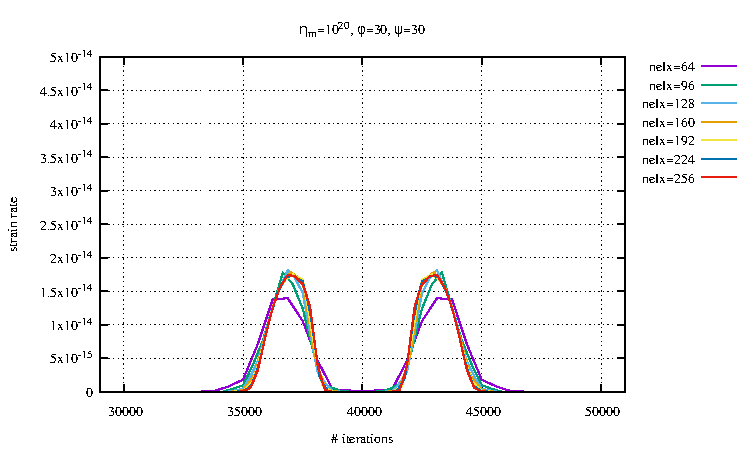
\includegraphics[width=.3\linewidth]{python_codes/fieldstone_39/benchmark1/extension/line_sr_phi30_psi30_etam20.pdf}\\
\end{center}
%\includegraphics[width=.3\linewidth]{python_codes/fieldstone_39/benchmark1/extension/line_eta_etam0.pdf}
%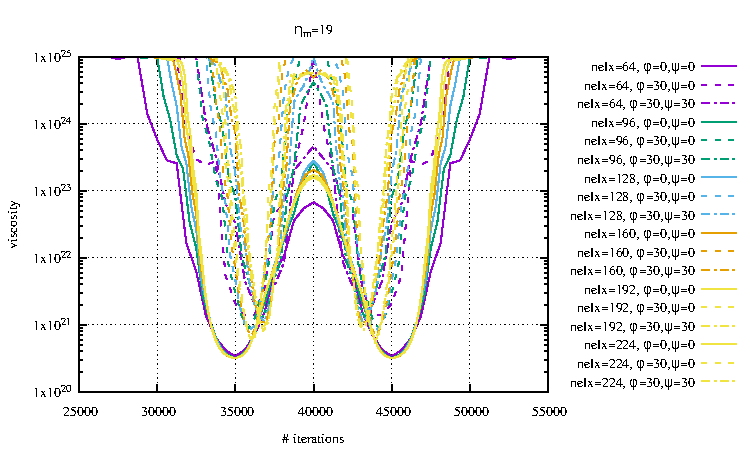
\includegraphics[width=.3\linewidth]{python_codes/fieldstone_39/benchmark1/extension/line_eta_etam19.pdf}
%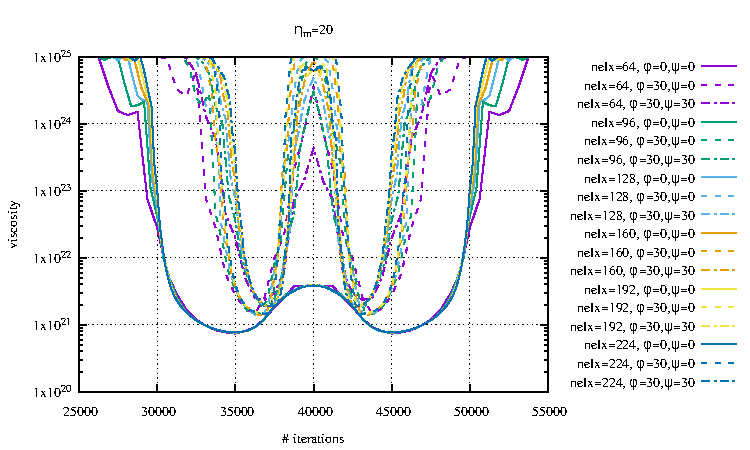
\includegraphics[width=.3\linewidth]{python_codes/fieldstone_39/benchmark1/extension/line_eta_etam20.pdf}\\

\newpage
\begin{center}
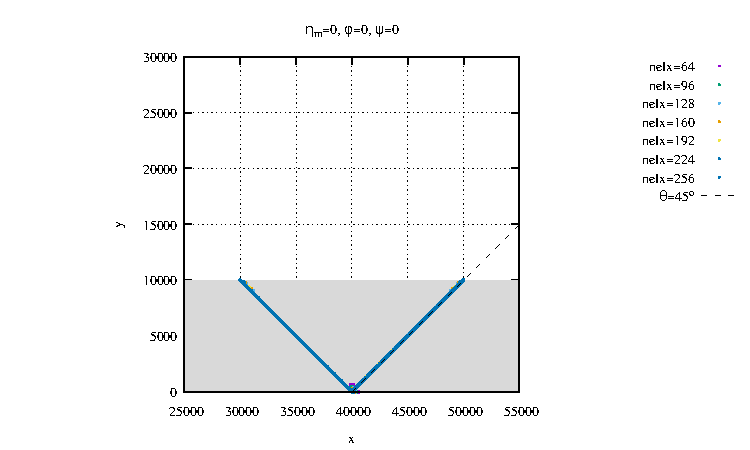
\includegraphics[width=.3\linewidth]{python_codes/fieldstone_39/benchmark1/extension/shear_band_phi0_psi0_etam0.pdf}
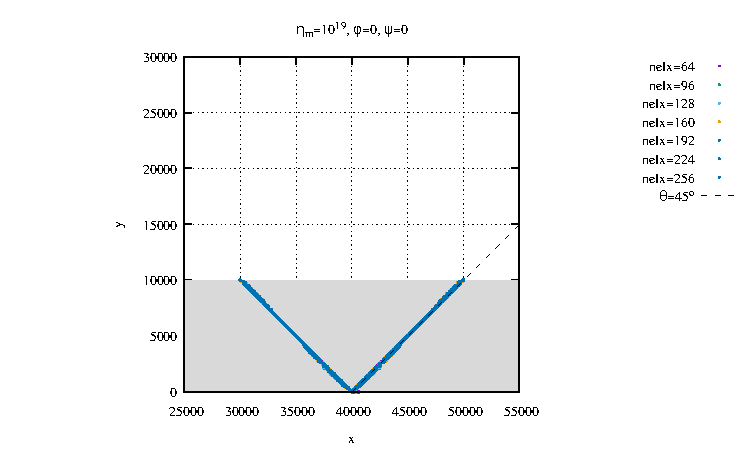
\includegraphics[width=.3\linewidth]{python_codes/fieldstone_39/benchmark1/extension/shear_band_phi0_psi0_etam19.pdf}
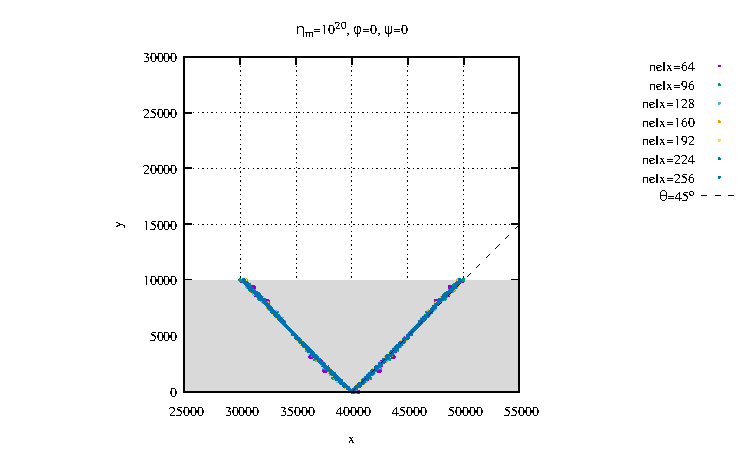
\includegraphics[width=.3\linewidth]{python_codes/fieldstone_39/benchmark1/extension/shear_band_phi0_psi0_etam20.pdf}\\
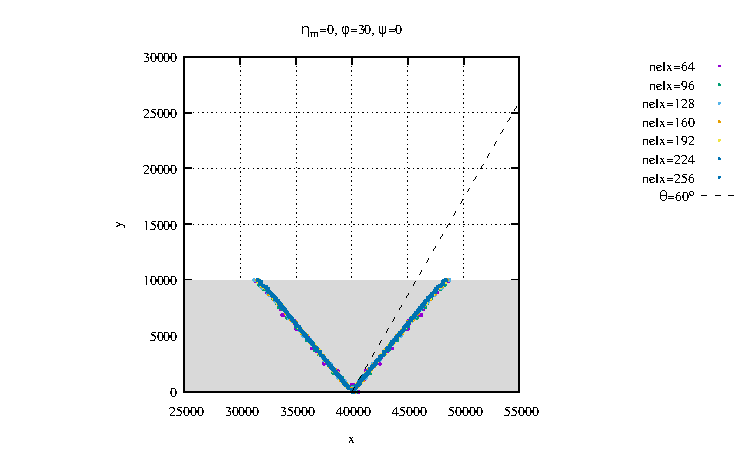
\includegraphics[width=.3\linewidth]{python_codes/fieldstone_39/benchmark1/extension/shear_band_phi30_psi0_etam0.pdf}
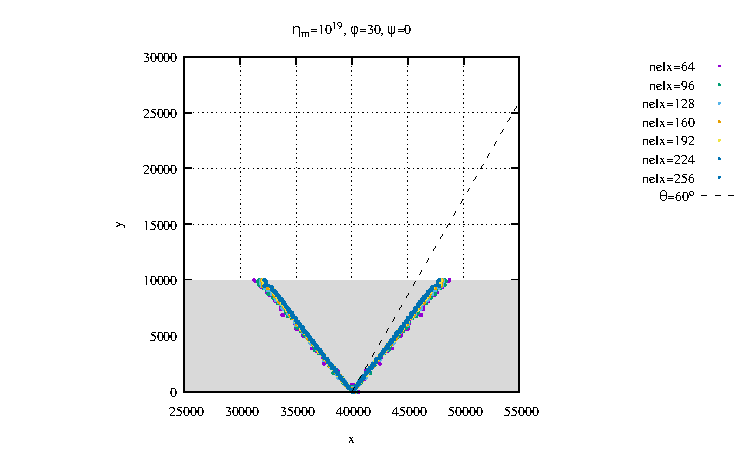
\includegraphics[width=.3\linewidth]{python_codes/fieldstone_39/benchmark1/extension/shear_band_phi30_psi0_etam19.pdf}
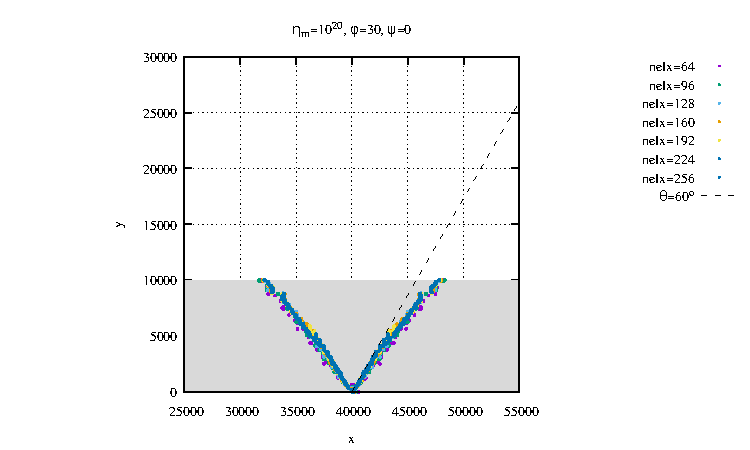
\includegraphics[width=.3\linewidth]{python_codes/fieldstone_39/benchmark1/extension/shear_band_phi30_psi0_etam20.pdf}\\
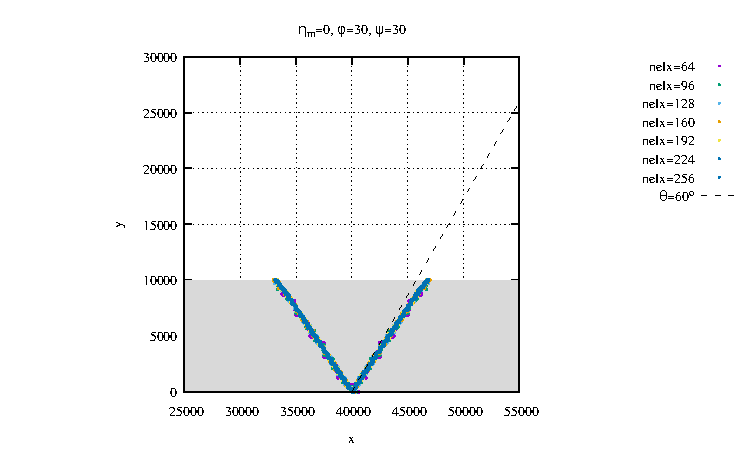
\includegraphics[width=.3\linewidth]{python_codes/fieldstone_39/benchmark1/extension/shear_band_phi30_psi30_etam0.pdf}
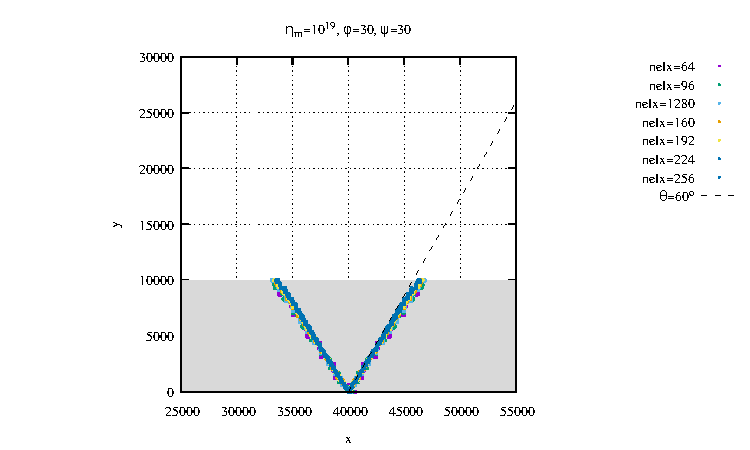
\includegraphics[width=.3\linewidth]{python_codes/fieldstone_39/benchmark1/extension/shear_band_phi30_psi30_etam19.pdf}
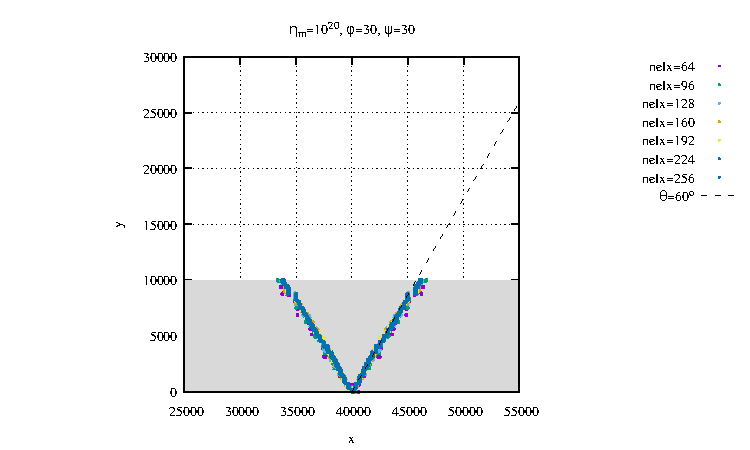
\includegraphics[width=.3\linewidth]{python_codes/fieldstone_39/benchmark1/extension/shear_band_phi30_psi30_etam20.pdf}
\end{center}


\newpage
One can also run the extension model for $\phi=\psi={0,5,10,15,20,25,30}\degree$:
\begin{center}
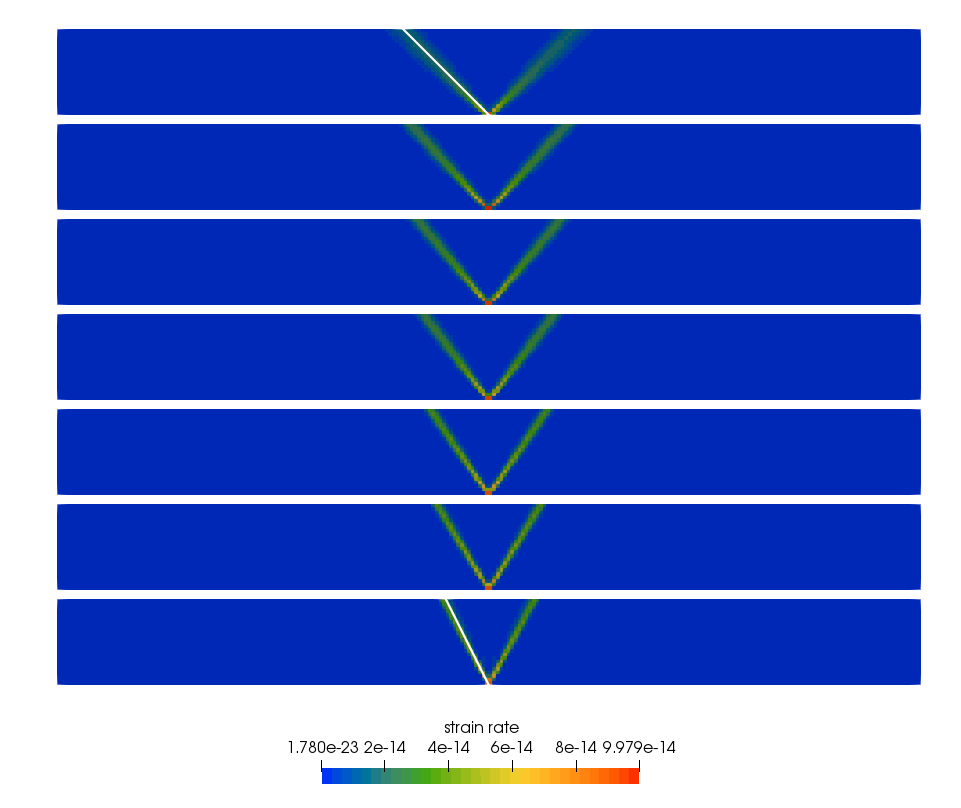
\includegraphics[width=.45\linewidth]{python_codes/fieldstone_39/images/sr_0_30}
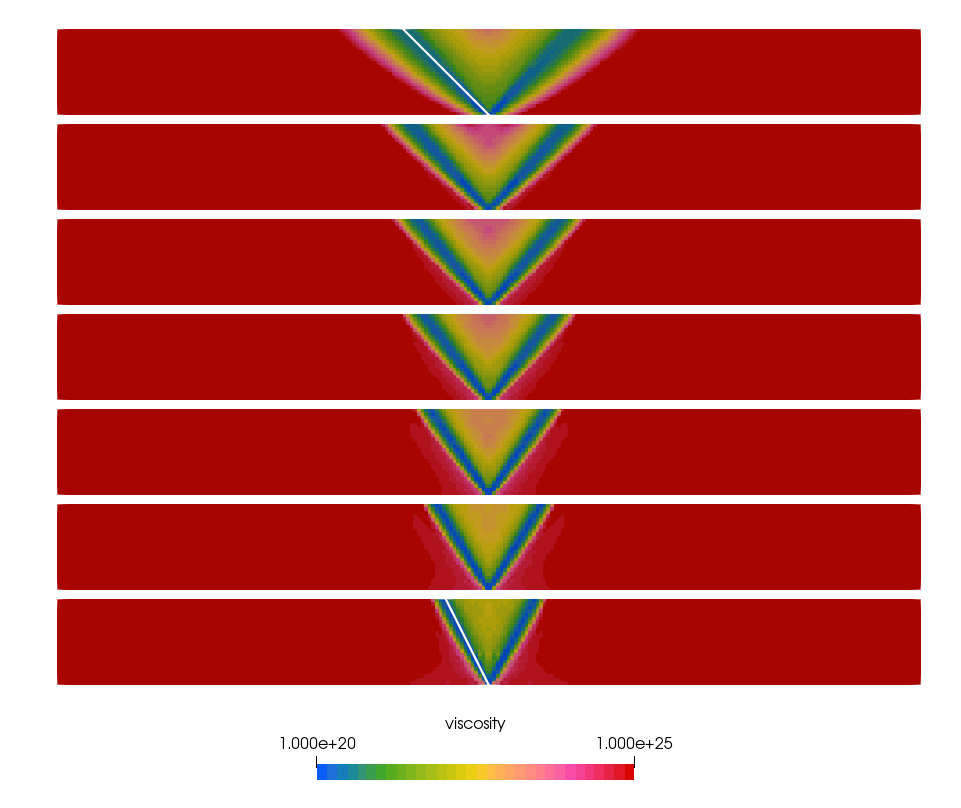
\includegraphics[width=.45\linewidth]{python_codes/fieldstone_39/images/etaeff_0_30}\\
\end{center}




\begin{center}
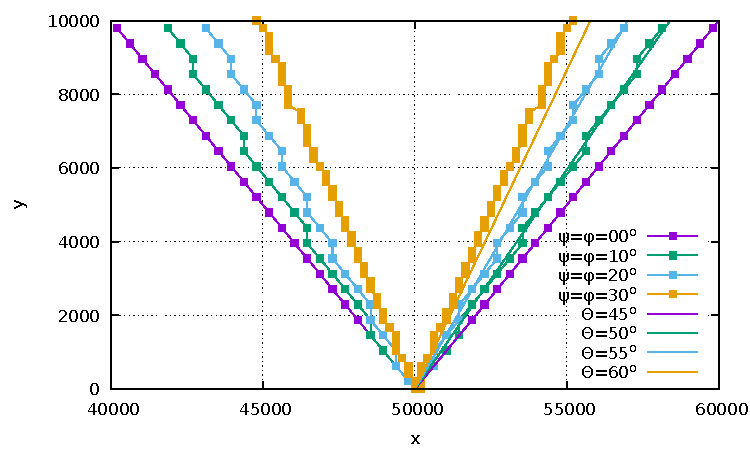
\includegraphics[width=.45\linewidth]{python_codes/fieldstone_39/images/shear_bands}
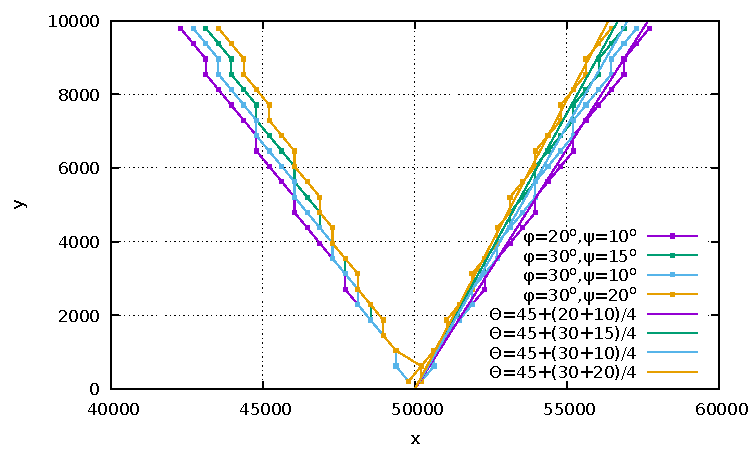
\includegraphics[width=.45\linewidth]{python_codes/fieldstone_39/images/shear_bands_nonass}\\
Results obtained on a 240x24 grid, max 50 nl iterations.
\end{center}


Note that benchmarking this in not easy. One solution Timo and I found was to add a 
velocity field $\underline{\vec\upnu}=(x,y,z)$ (with $\vec\nabla\cdot\underline{\vec\upnu}=3$)
to an existing analytical problem, e.g. the Burstedde benchamrk.

\newpage
%...........................................................
\subsection*{Benchmark \#2 - Spiegelman et al (2016) brick}

The setup is {\sl similar} to the one in Spiegelman et al (2016) \cite{spmw16}. 
It is a 2D Cartesian domain filled with an 
isoviscous layer at the bottom and a visco-plastic material on top, as shown here:  

\begin{center}
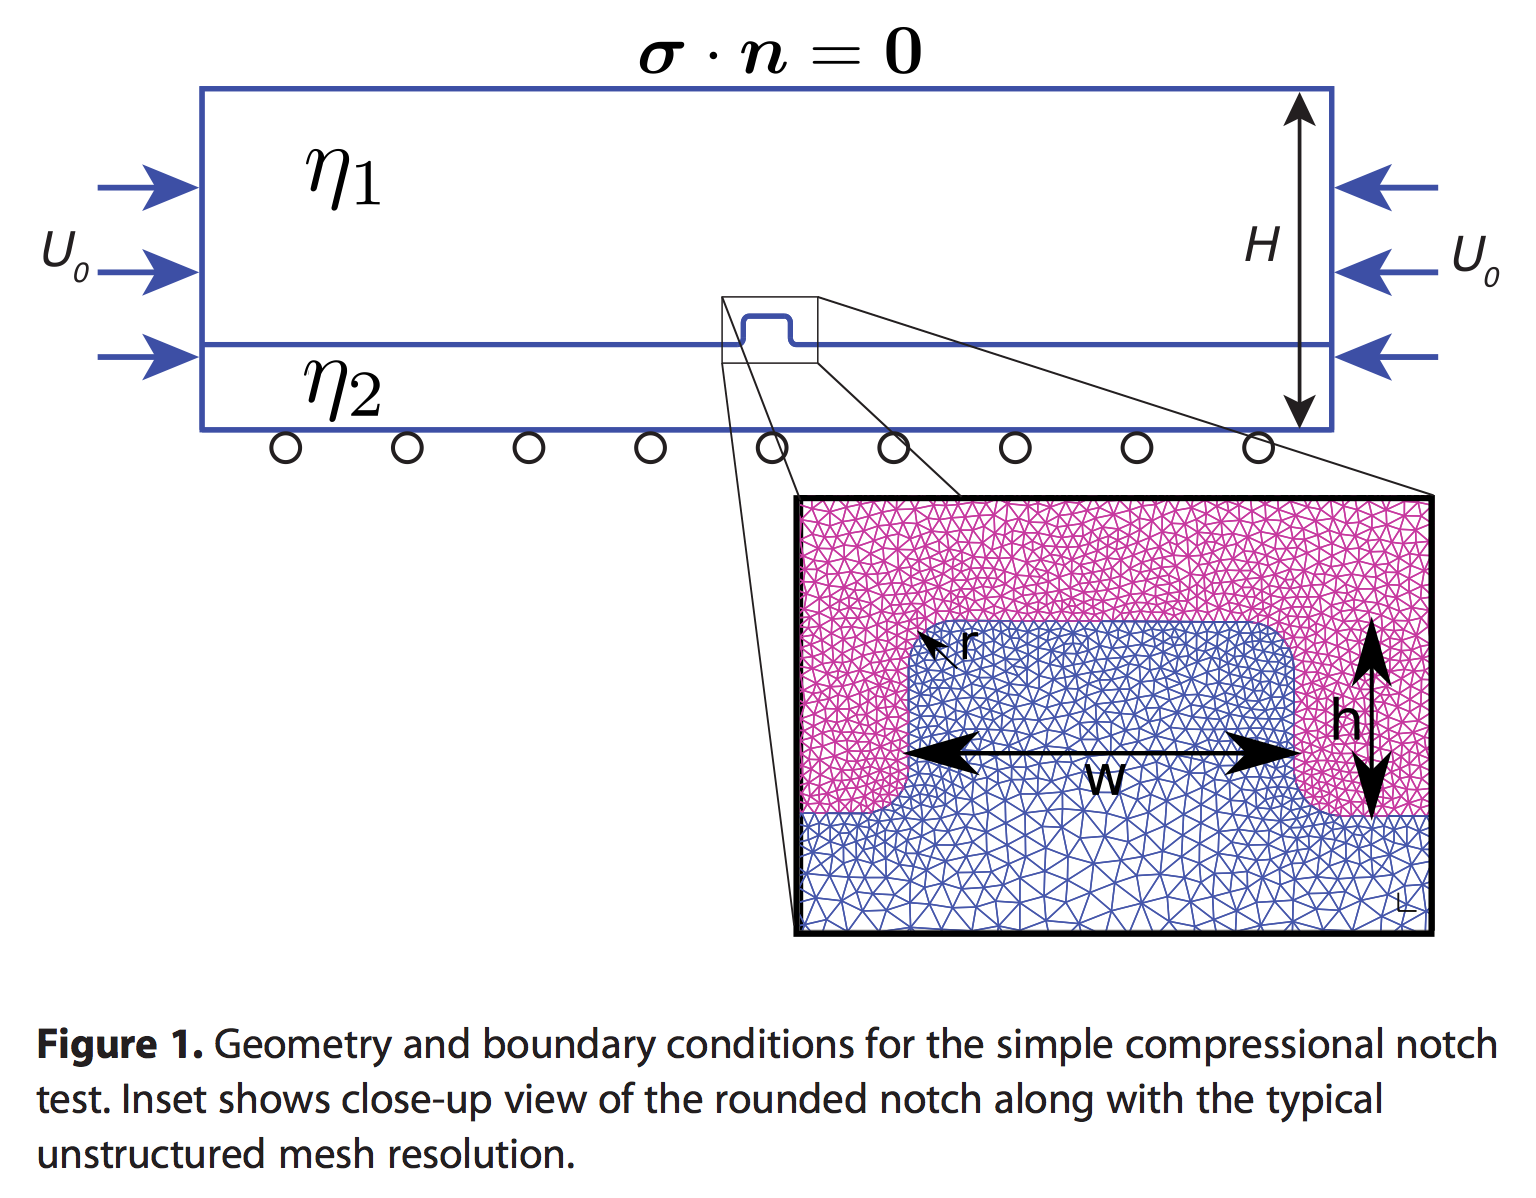
\includegraphics[width=6cm]{python_codes/fieldstone_39/images/spmw_1.png}
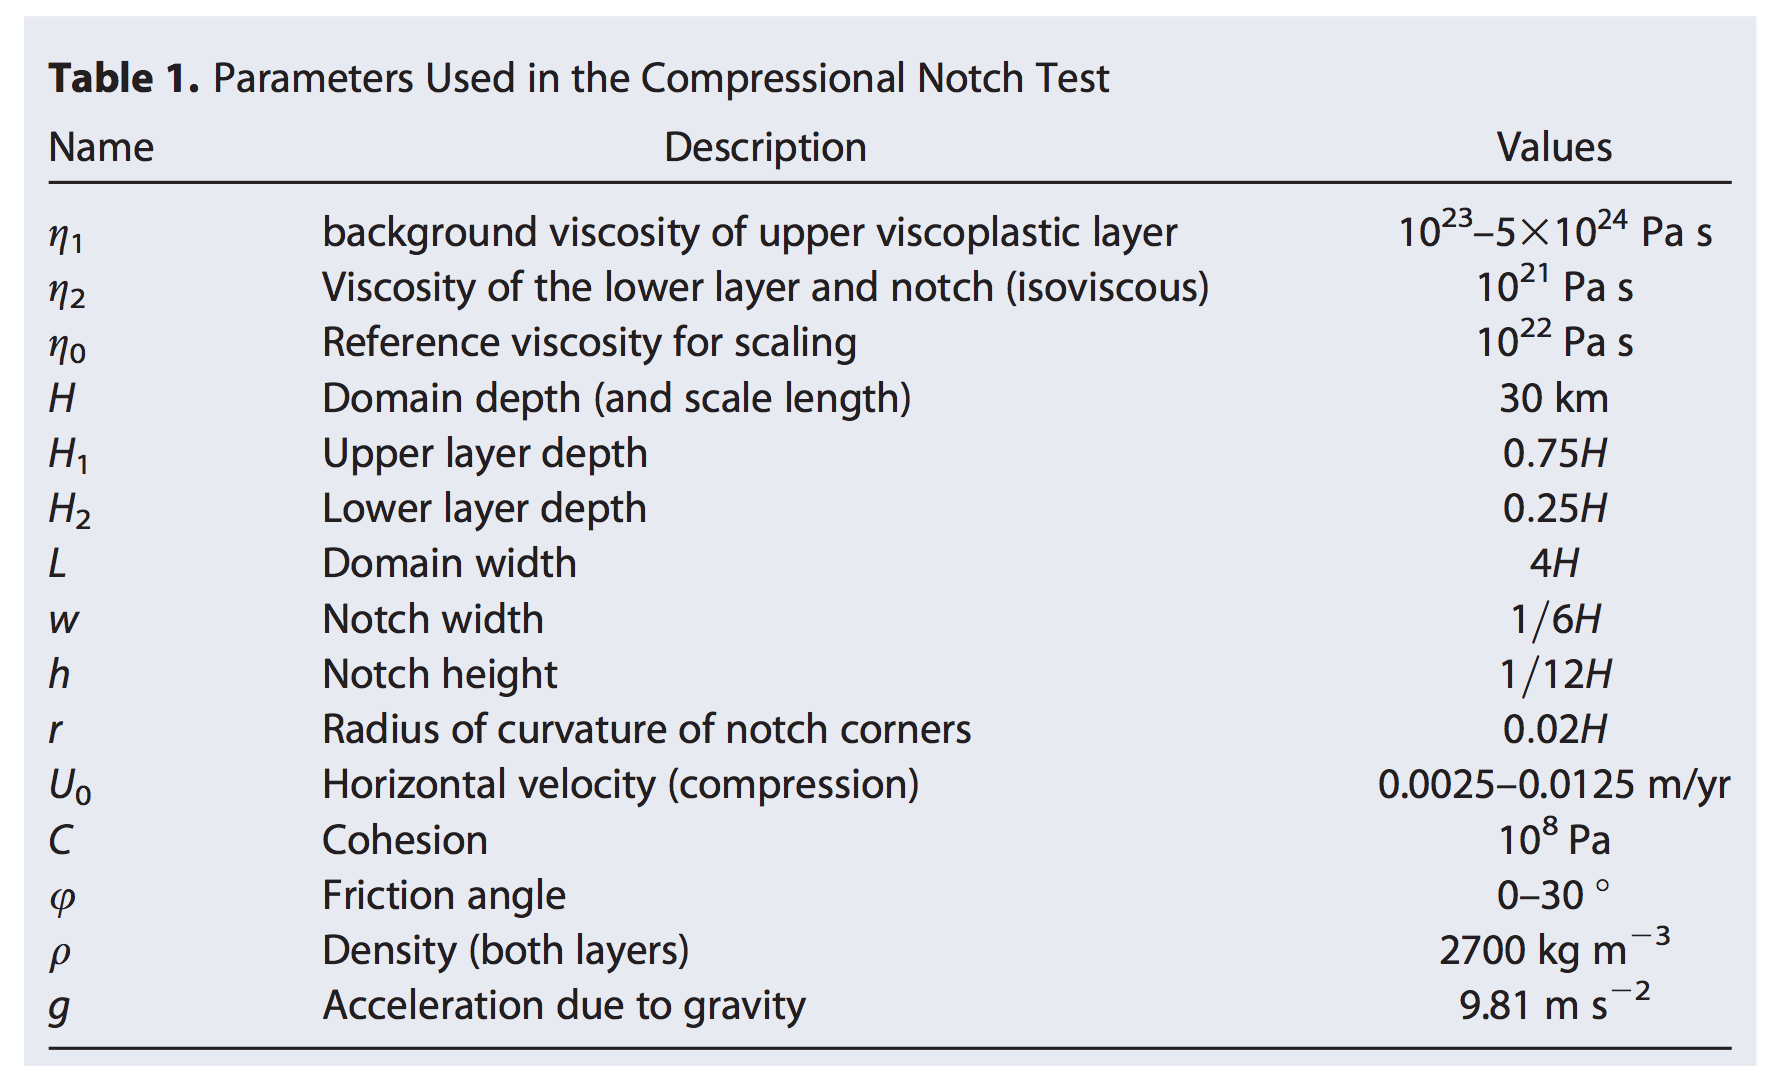
\includegraphics[width=8cm]{python_codes/fieldstone_39/images/spmw_2.png}
\end{center}

The domain has dimensions $L_x=128\si{\kilo\metre}$, $L_y=Lx/4$. 
The lower layer depth is $L_y/4$. The notch has dimensions $w=4\si{\kilo\metre}$
and $h=2\si{\kilo\metre}$. 

In what follows the nonlinear tolerance is set to $10^{-6}$. Due to a lack of resolution, I do not
implement the rounded edges of the seed. $U_0$ is set to $25\si{\mm\per\year}$ 
and the background viscosity of the brittle layer
is set to $\eta_v=10^{24}\si{\pascal\second}$. 

Note that the pressure colour bars in Fig(6) of \cite{spmw16} are most likely not correct at all: 
\begin{center}
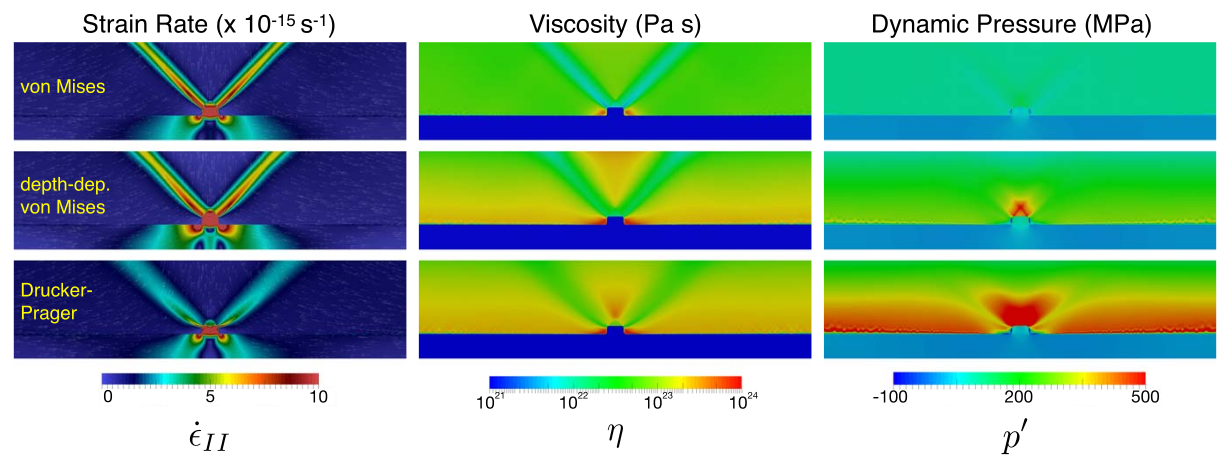
\includegraphics[width=12cm]{python_codes/fieldstone_39/images/spmw_3.png}\\
{\captionfont Fig.(6) from Spiegelman et al (2016) \cite{spmw16}.}
\end{center}





\newpage
%........................................................
\subsection*{Benchmark \#4: Shortening of a visco-plastic bloc - part 1}

This benchmark originates in the book of Gerya. In the first edition the domain is 1000x1000km, 
while it is 100x100km in the second. We keep the second edition as a guideline. The benchmark
is actually elasto-visco-plastic but in this stone we neglect the elastic deformation. The 
boundary conditions are shown here:

\begin{center}
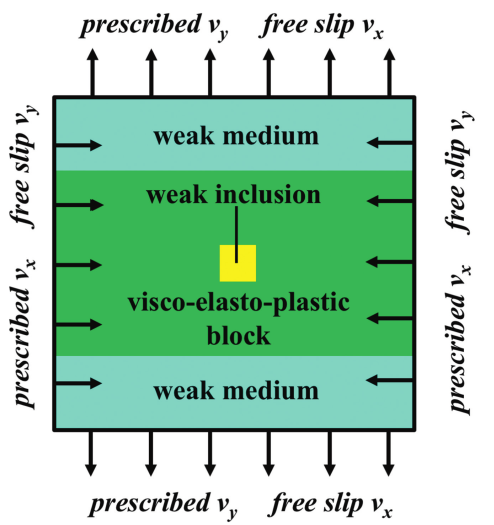
\includegraphics[width=6cm]{python_codes/fieldstone_39/results_shortening_block/setup}\\
{\captionfont Taken from \cite{gery19book}.}
\end{center}

The velocity on the boundaries is $\upnu_{bc}=5\cdot 10^{-9}$ \si{\metre\per\second} so that the background strain rate is 
$2 \upnu_{bc}/L = 10^{-13}\si{\per\second}$.
The weak medium and the weak inclusion have a viscosity $\eta=10^{17}\si{\pascal\second}$ while 
the block is visco-plastic, with $\eta=10^{23}\si{\pascal\second}$, $c=10^8\si{\pascal}$ 
and $\phi=37\degree$. 
Pressure is set to zero in the top right corner and later post-processed so as to insure a zero 
volume average.

In the case of von Mises ($\phi=0$) we expect the shear bands at $45\degree$. When $\phi>0$, as mentioned above
we expect:
\[
\frac{\pi}{4}-\frac{\phi}{2}=26.5\degree
\qquad
\frac{\pi}{4}-\frac{\phi}{4}=35.75\degree
\]

\begin{center}
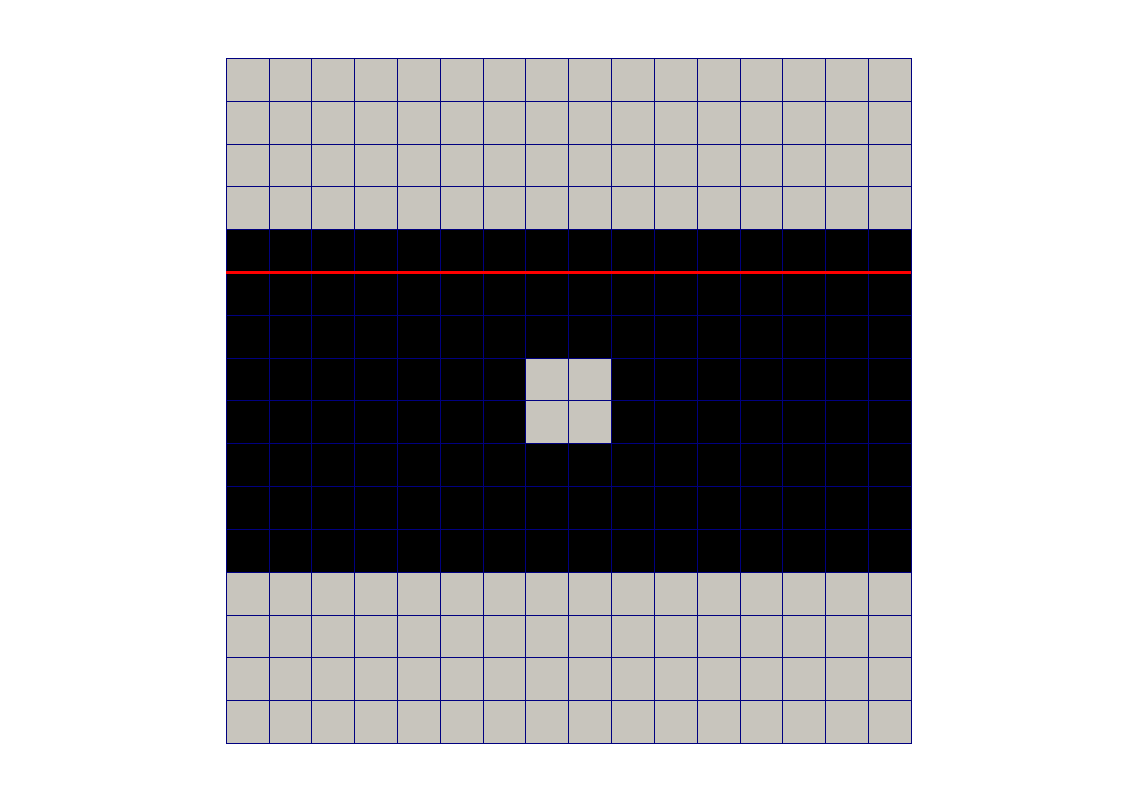
\includegraphics[width=8cm]{python_codes/fieldstone_39/results_shortening_block/line}
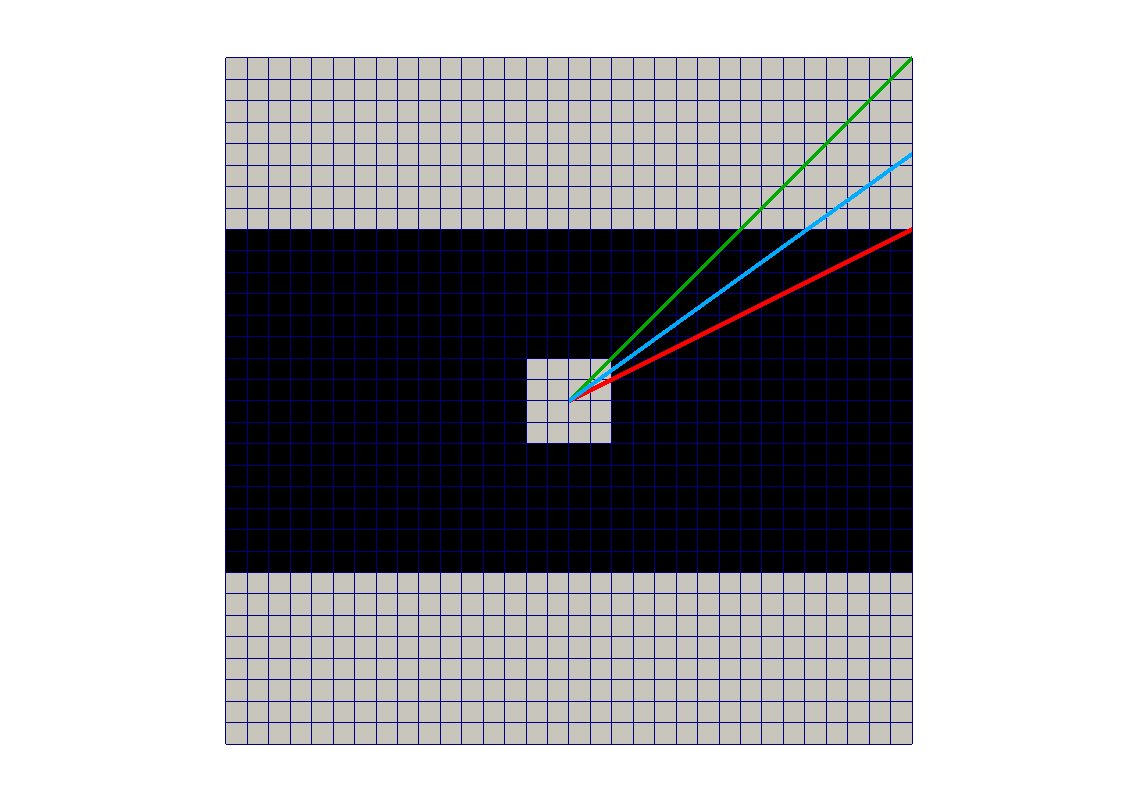
\includegraphics[width=8cm]{python_codes/fieldstone_39/results_shortening_block/angles}\\
{\captionfont a) Line on which strain rate is measured. b) possible shear band angles:
green is $45\degree$, blue is $35.75\degree$ and red is $26.5\degree$.}
\end{center}


I have adapted slightly the dimensions inside the domain such that resolutions 16x16, 32x32, etc...
all showcase elements whose sides exactly align with the material interfaces. The size of the inclusion is 
$L/8=12.5$km and the block has a thickness of 50km:

\begin{center}
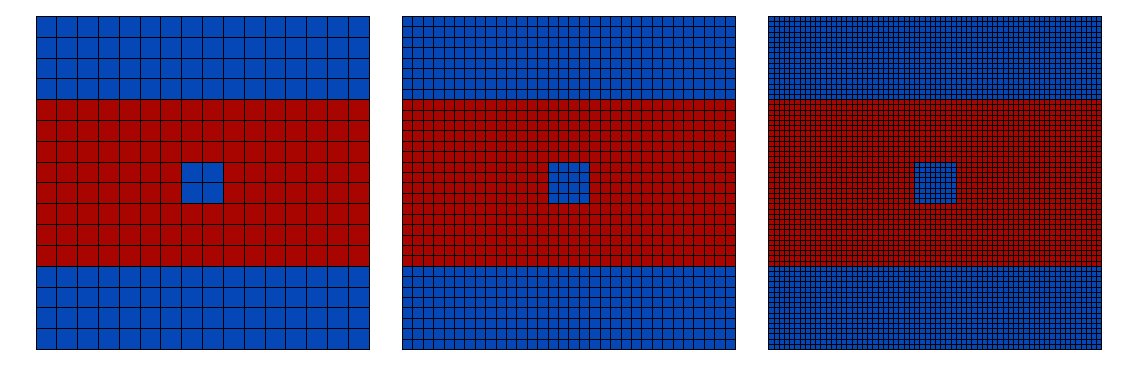
\includegraphics[width=10cm]{python_codes/fieldstone_39/results_shortening_block/geometry}\\
{\captionfont Material geometry for resolutions 16x16, 32x32 and 64x64.}
\end{center}


\newpage
\underline{von Mises (no dilation rate):}

\begin{center}
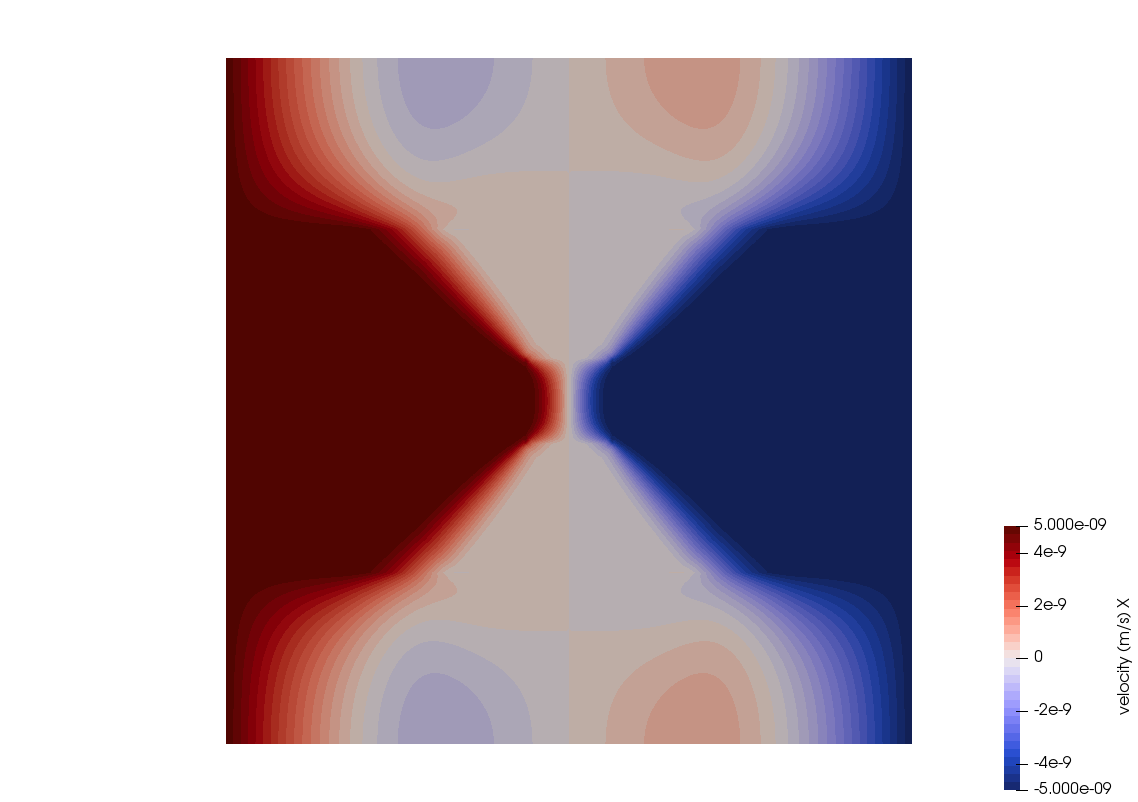
\includegraphics[width=5cm]{python_codes/fieldstone_39/results_shortening_block/u}
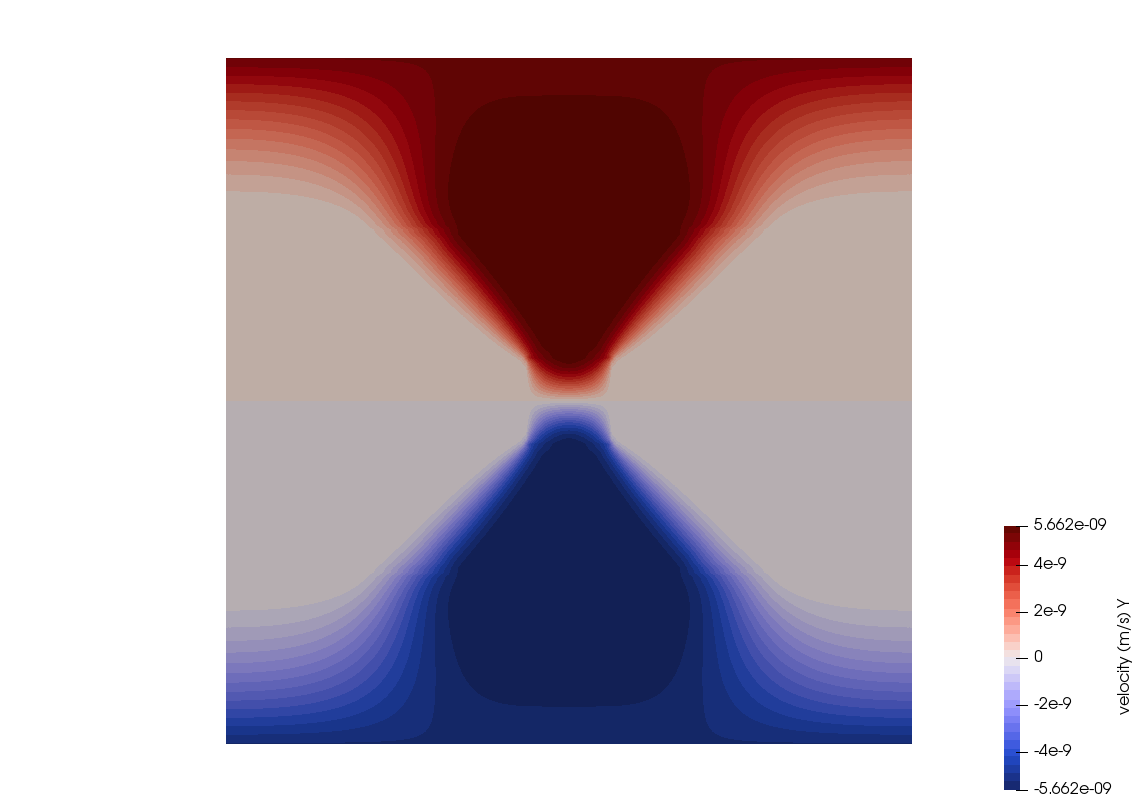
\includegraphics[width=5cm]{python_codes/fieldstone_39/results_shortening_block/v}
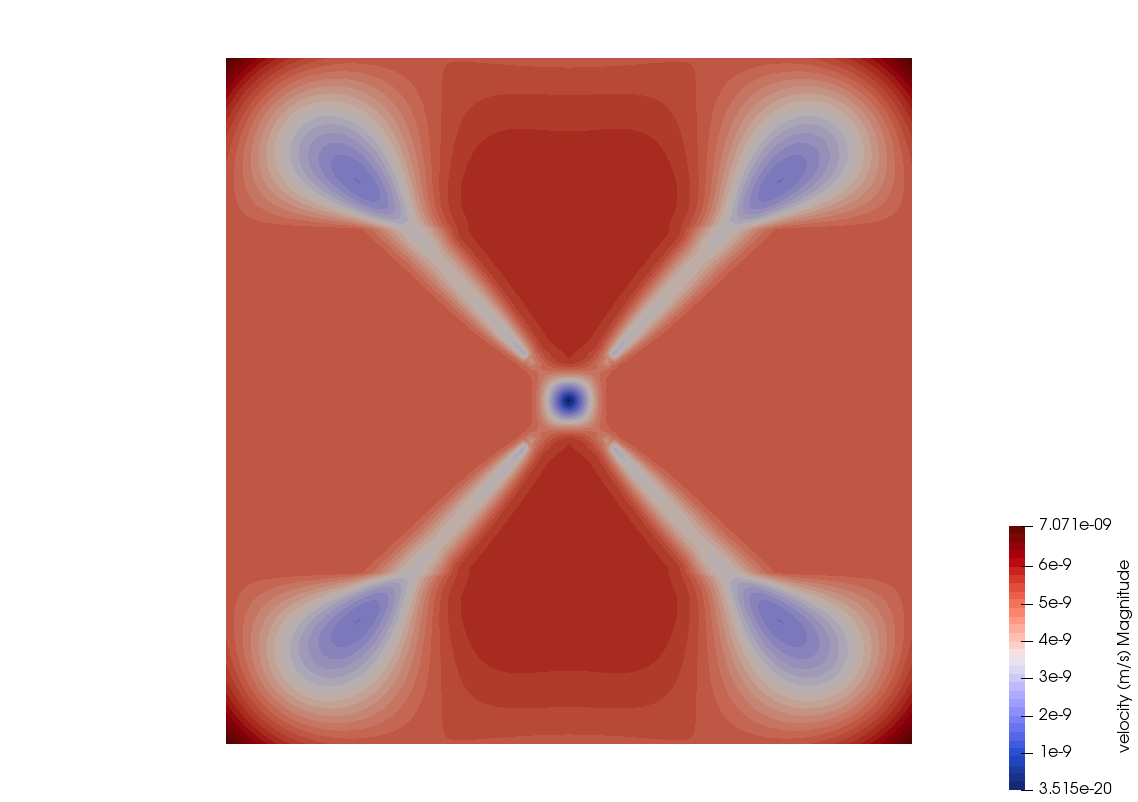
\includegraphics[width=5cm]{python_codes/fieldstone_39/results_shortening_block/vel}\\
{\captionfont Velocity field for 128x128, $\eta_m=1e19$}
\end{center}

\begin{center}
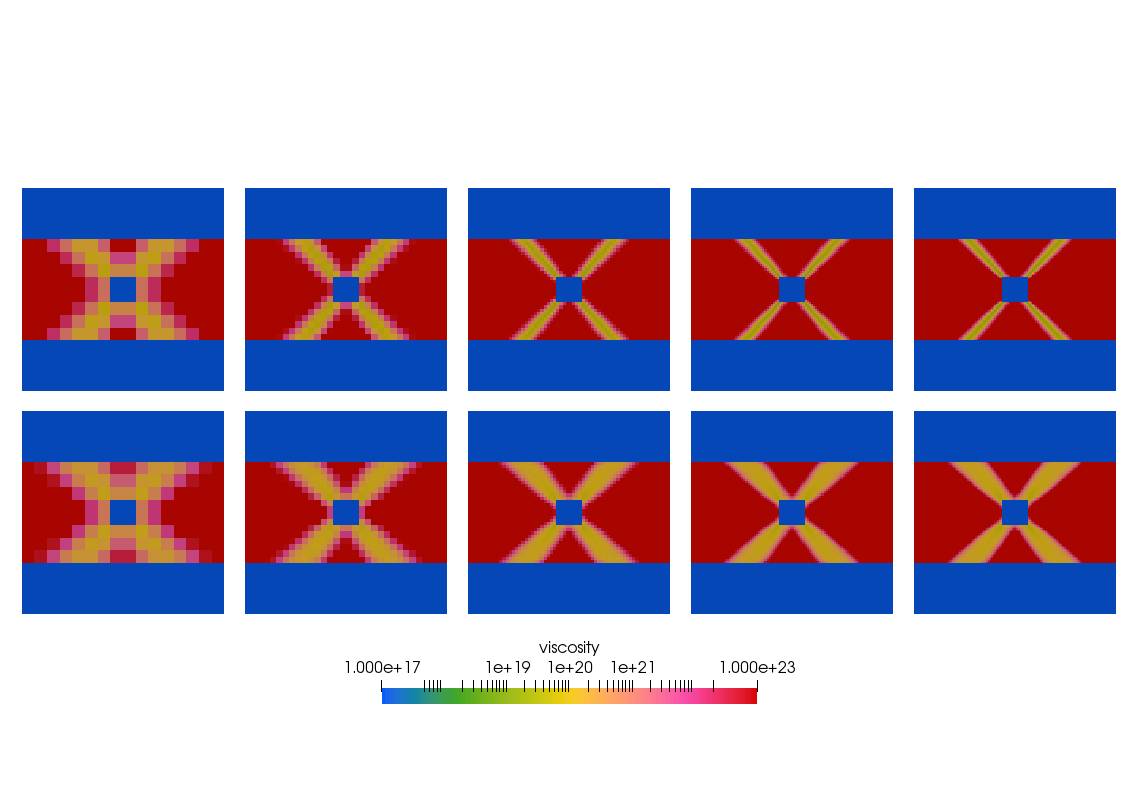
\includegraphics[width=8cm]{python_codes/fieldstone_39/results_shortening_block/etaeff}
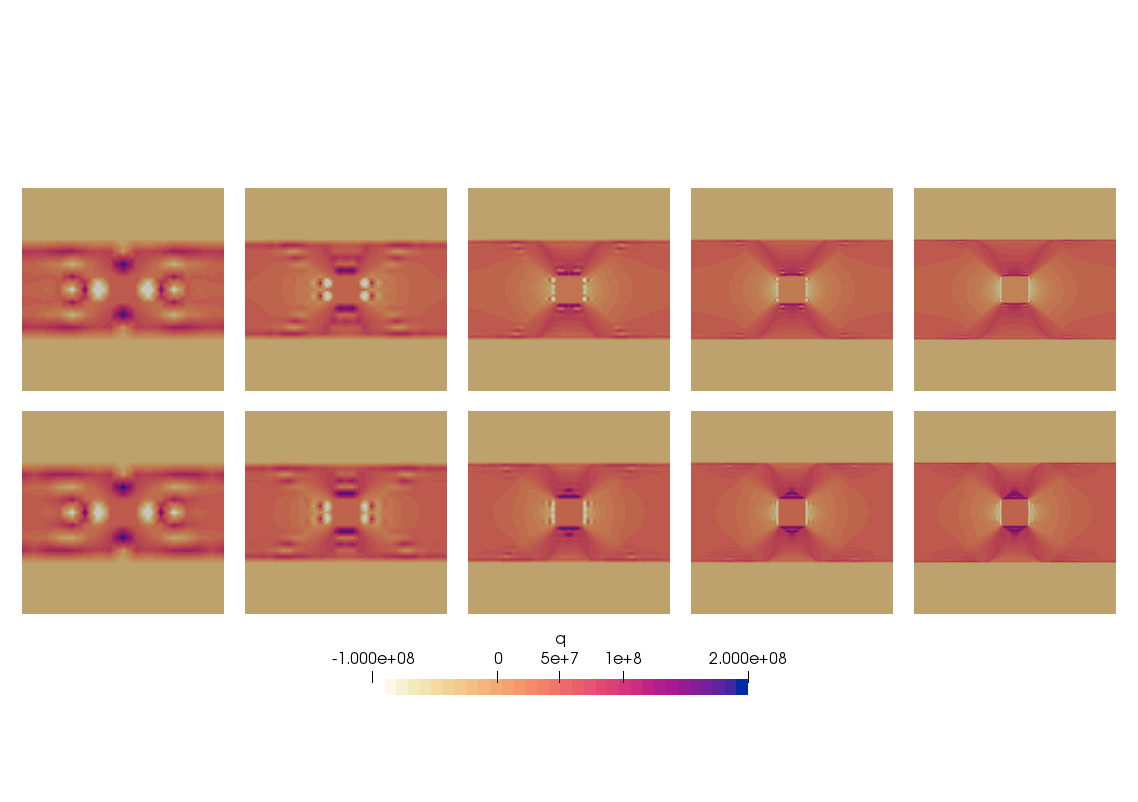
\includegraphics[width=8cm]{python_codes/fieldstone_39/results_shortening_block/p}\\
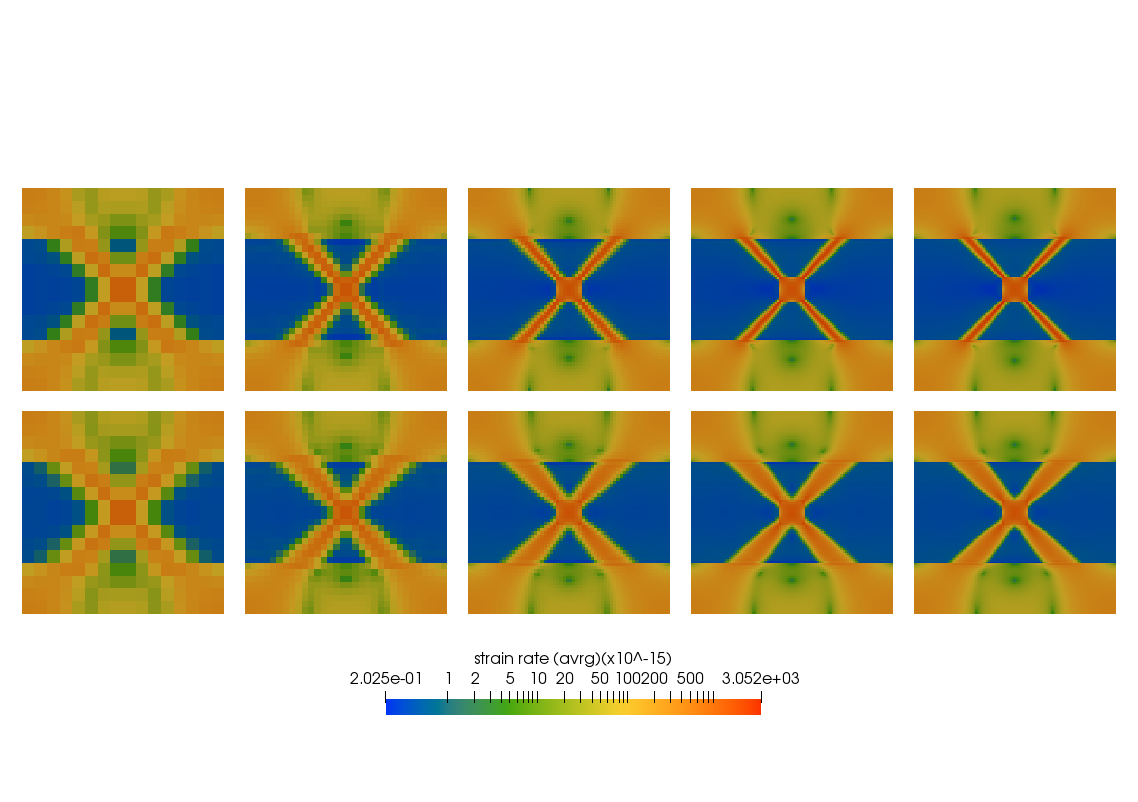
\includegraphics[width=8cm]{python_codes/fieldstone_39/results_shortening_block/sr_elt_log}
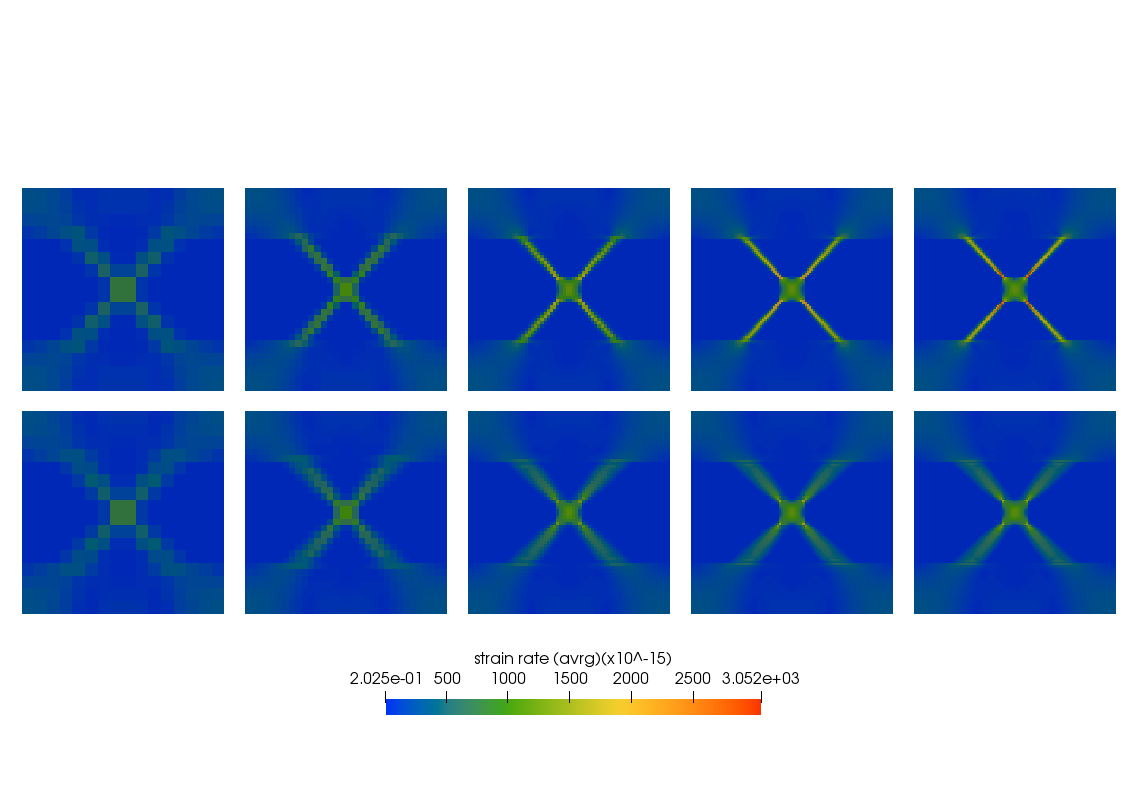
\includegraphics[width=8cm]{python_codes/fieldstone_39/results_shortening_block/sr_elt}\\
{\captionfont From left to right: resolutions are 16x16, 32x32, 64x64 and 96x96. 100 nonlinear Picard iterations.}
\end{center}

\begin{center}
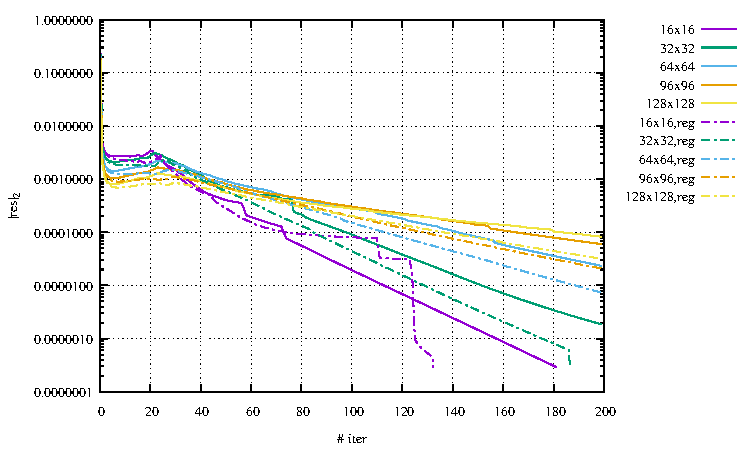
\includegraphics[width=5cm]{python_codes/fieldstone_39/results_shortening_block/conv_vM.pdf}
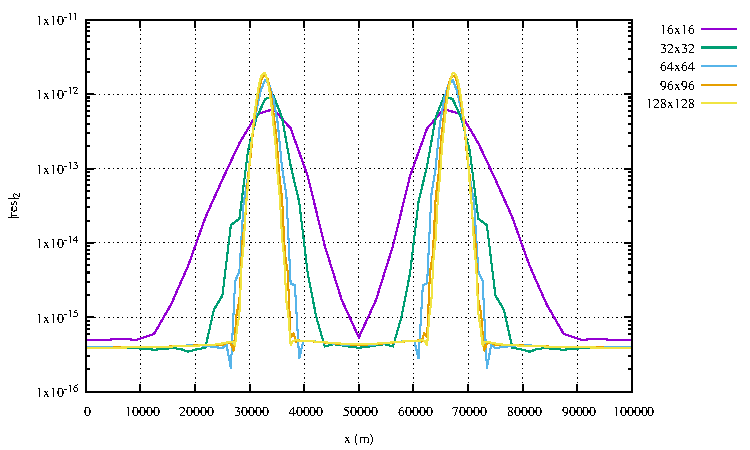
\includegraphics[width=5cm]{python_codes/fieldstone_39/results_shortening_block/sr_line_vM.pdf}
\includegraphics[width=5cm]{python_codes/fieldstone_39/results_shortening_block/sr_line_vM_reg.pdf}\\
{\captionfont $\eta_m=1e19$}
\end{center}




\newpage
\underline{viscous damper, no dilation rate, Drucker-Prager, phi=37:}


\begin{center}
\includegraphics[width=8cm]{python_codes/fieldstone_39/results_shortening_block/conv_DP.pdf}
\includegraphics[width=8cm]{python_codes/fieldstone_39/results_shortening_block/conv_DP_1e19.pdf}\\
{\captionfont Left: $\eta_m=0$, right: $\eta_m=10^{19}$}
\end{center}


\begin{center}
\includegraphics[width=4cm]{python_codes/fieldstone_39/results_shortening_block/32x32_phi37_1e19/sr}
\includegraphics[width=4cm]{python_codes/fieldstone_39/results_shortening_block/32x32_phi37_1e19/sr_log}
\includegraphics[width=4cm]{python_codes/fieldstone_39/results_shortening_block/32x32_phi37_1e19/p}
\includegraphics[width=4cm]{python_codes/fieldstone_39/results_shortening_block/32x32_phi37_1e19/eta}\\
{\captionfont Fieldstone 32x32}\\
\includegraphics[width=4cm]{python_codes/fieldstone_39/results_shortening_block/aspect_32x32_1e19_phi37/sr}
\includegraphics[width=4cm]{python_codes/fieldstone_39/results_shortening_block/aspect_32x32_1e19_phi37/sr_log}
\includegraphics[width=4cm]{python_codes/fieldstone_39/results_shortening_block/aspect_32x32_1e19_phi37/p}
\includegraphics[width=4cm]{python_codes/fieldstone_39/results_shortening_block/aspect_32x32_1e19_phi37/eta}\\
\includegraphics[width=4cm]{python_codes/fieldstone_39/results_shortening_block/aspect_64x64_1e19_phi37/sr}
\includegraphics[width=4cm]{python_codes/fieldstone_39/results_shortening_block/aspect_64x64_1e19_phi37/sr_log}
\includegraphics[width=4cm]{python_codes/fieldstone_39/results_shortening_block/aspect_64x64_1e19_phi37/p}
\includegraphics[width=4cm]{python_codes/fieldstone_39/results_shortening_block/aspect_64x64_1e19_phi37/eta}\\
{\captionfont ASPECT 32x32, 64x64} 
\end{center}



\newpage
To explore:

- associative and non-associative drucker-prage

- visco-plastic vs visco-viscoplastic







\newpage
%..............................................
\subsection*{Benchmark \#5: Shortening of a visco-plastic bloc - part 2}

The setup originates in Duretz et al (2018) \cite{dusd18} and is also carried out 
in Jacquey \& Cacace (2020) \cite{jaca20a}. We here again neglect the elastic 
deformation. 
The domain is 4x2 km. There is a linear viscous inclusion in the middle of radius 100\si{\metre} and 
viscosity $\eta_{inc}=10^{17}\si{\pascal\second}$. The material around is characterised by 
$\eta_v=10^{24}\si{pascal\second}$, $c=3e7\si{pascal}$, $\phi=30\degree$, $psi=10\degree$.
Boundary conditions are as follows: 

\begin{center}
\includegraphics[width=6cm]{python_codes/fieldstone_39/results_shortening_block2/jaca20a}
\end{center}

In the papers they prescribe $\Delta \varepsilon = 5\cdot 10^{-5}$ over a 
time step of $\Delta t=10^{10}\si{second}$, 
i.e. the background strain rate is $\dot\varepsilon=5\cdot 10^{-15}\si{\per\second}$.
Given $L_x$ and $L_y$ we can easily arrive at the velocity values to be prescribed:
\[
|u_{bc}|=\dot{\varepsilon}_{bc} L_x/2
\qquad
|v_{bc}|=\dot{\varepsilon}_{bc} L_y/2
\]
 
The inclusion is circular, i.e. no amount of mesh refinement will be such that the mesh 
edges align with it, as opposed to the previous experiment. 


\begin{center}
\includegraphics[width=8cm]{python_codes/fieldstone_39/results_shortening_block2/dusd18}
\includegraphics[width=8cm]{python_codes/fieldstone_39/results_shortening_block2/jaca20b}\\
{\captionfont Left: taken from Duretz et al (2018) \cite{dusd18}; Right: taken from Jacquey \& Cacace (2020) \cite{jaca20a}.
Note that these simulations have been run with elasto-visco-plastic rheologies 
for a certain amount of time so that the propagation of the shear bands is not final/complete, as
opposed to the converged visco-plastic solutions shown hereafter.}
\end{center}

As before, pressure is set to zero in the top right corner, and further post processed to insure that its volume 
average is zero.


\clearpage
\subsubsection*{von Mises rheology}

\begin{center}
\includegraphics[width=8cm]{python_codes/fieldstone_39/results_shortening_block2/conv_vM}\\
{\captionfont Nonlinear convergence, fieldstone and aspect, 128x64, 200 nonlinear iterations, $\eta_m=10^{19}$.}
\end{center}
\begin{center}
\includegraphics[width=5.8cm]{python_codes/fieldstone_39/results_shortening_block2/128x64_1e19/u}
\includegraphics[width=5.8cm]{python_codes/fieldstone_39/results_shortening_block2/128x64_1e19/v}
\includegraphics[width=5.8cm]{python_codes/fieldstone_39/results_shortening_block2/128x64_1e19/vel}\\
\includegraphics[width=5.8cm]{python_codes/fieldstone_39/results_shortening_block2/128x64_1e19/eta}
\includegraphics[width=5.8cm]{python_codes/fieldstone_39/results_shortening_block2/128x64_1e19/sr}
\includegraphics[width=5.8cm]{python_codes/fieldstone_39/results_shortening_block2/128x64_1e19/p}\\
{\captionfont 128x64, 200 nonlinear iterations, $\eta_m=10^{19}$}
\end{center}

\begin{center}
\includegraphics[width=5.8cm]{python_codes/fieldstone_39/results_shortening_block2/aspect_128x64_1e19/u}
\includegraphics[width=5.8cm]{python_codes/fieldstone_39/results_shortening_block2/aspect_128x64_1e19/v}
\includegraphics[width=5.8cm]{python_codes/fieldstone_39/results_shortening_block2/aspect_128x64_1e19/vel}\\
\includegraphics[width=5.8cm]{python_codes/fieldstone_39/results_shortening_block2/aspect_128x64_1e19/eta}
\includegraphics[width=5.8cm]{python_codes/fieldstone_39/results_shortening_block2/aspect_128x64_1e19/sr}
\includegraphics[width=5.8cm]{python_codes/fieldstone_39/results_shortening_block2/aspect_128x64_1e19/p}\\
{\captionfont ASPECT: 128x64, 200 nonlinear iterations, $\eta_m=10^{19}$}
\end{center}

\newpage
In order to help the comparison, I plot the effective viscosity and the strain rate for both next to one another:
\begin{center}
\includegraphics[width=8cm]{python_codes/fieldstone_39/results_shortening_block2/eta_both}
\includegraphics[width=8cm]{python_codes/fieldstone_39/results_shortening_block2/sr_both}\\
{\captionfont Left half is fieldstone, Right half is aspect.}
\end{center}


\begin{center}
\includegraphics[width=10cm]{python_codes/fieldstone_39/results_shortening_block2/sr_line_vM.pdf}\\
{\captionfont Strain rate cross section at $y=11L_y/16$.}
\end{center}


\clearpage
\subsubsection*{Drucker-Prager rheology ($\phi=30\degree$)}

\includegraphics[width=8cm]{python_codes/fieldstone_39/results_shortening_block2/conv_DP}
\includegraphics[width=8cm]{python_codes/fieldstone_39/results_shortening_block2/sr_line_DP.pdf}

\begin{center}
\includegraphics[width=4cm]{python_codes/fieldstone_39/results_shortening_block2/32x16_1e19_phi30/vel}
\includegraphics[width=4cm]{python_codes/fieldstone_39/results_shortening_block2/32x16_1e19_phi30/p}
\includegraphics[width=4cm]{python_codes/fieldstone_39/results_shortening_block2/32x16_1e19_phi30/sr}
\includegraphics[width=4cm]{python_codes/fieldstone_39/results_shortening_block2/32x16_1e19_phi30/eta}\\
\includegraphics[width=4cm]{python_codes/fieldstone_39/results_shortening_block2/48x24_1e19_phi30/vel}
\includegraphics[width=4cm]{python_codes/fieldstone_39/results_shortening_block2/48x24_1e19_phi30/p}
\includegraphics[width=4cm]{python_codes/fieldstone_39/results_shortening_block2/48x24_1e19_phi30/sr}
\includegraphics[width=4cm]{python_codes/fieldstone_39/results_shortening_block2/48x24_1e19_phi30/eta}\\
\includegraphics[width=4cm]{python_codes/fieldstone_39/results_shortening_block2/64x32_1e19_phi30/vel}
\includegraphics[width=4cm]{python_codes/fieldstone_39/results_shortening_block2/64x32_1e19_phi30/p}
\includegraphics[width=4cm]{python_codes/fieldstone_39/results_shortening_block2/64x32_1e19_phi30/sr}
\includegraphics[width=4cm]{python_codes/fieldstone_39/results_shortening_block2/64x32_1e19_phi30/eta}\\
\includegraphics[width=4cm]{python_codes/fieldstone_39/results_shortening_block2/128x64_1e19_phi30/vel}
\includegraphics[width=4cm]{python_codes/fieldstone_39/results_shortening_block2/128x64_1e19_phi30/p}
\includegraphics[width=4cm]{python_codes/fieldstone_39/results_shortening_block2/128x64_1e19_phi30/sr}
\includegraphics[width=4cm]{python_codes/fieldstone_39/results_shortening_block2/128x64_1e19_phi30/eta}\\
{\captionfont Fielstone. Top to bottom: 32x16, 48x24, 64x32, 128x64, etam=1e19, phi=30}\\
\includegraphics[width=4cm]{python_codes/fieldstone_39/results_shortening_block2/aspect_32x16_1e19_phi30/vel}
\includegraphics[width=4cm]{python_codes/fieldstone_39/results_shortening_block2/aspect_32x16_1e19_phi30/p}
\includegraphics[width=4cm]{python_codes/fieldstone_39/results_shortening_block2/aspect_32x16_1e19_phi30/sr}
\includegraphics[width=4cm]{python_codes/fieldstone_39/results_shortening_block2/aspect_32x16_1e19_phi30/eta}\\
\includegraphics[width=4cm]{python_codes/fieldstone_39/results_shortening_block2/aspect_64x32_1e19_phi30/vel}
\includegraphics[width=4cm]{python_codes/fieldstone_39/results_shortening_block2/aspect_64x32_1e19_phi30/p}
\includegraphics[width=4cm]{python_codes/fieldstone_39/results_shortening_block2/aspect_64x32_1e19_phi30/sr}
\includegraphics[width=4cm]{python_codes/fieldstone_39/results_shortening_block2/aspect_64x32_1e19_phi30/eta}\\
{\captionfont ASPECT, 64x32, etam=1e19, phi=30}\\
\end{center}

Note that ASPECT does not use the proper partitioning of strain rates, and uses total strain rate 
in plastic element. This could explain the difference?



\clearpage
\subsubsection*{A very different approach: diffusion plasticity}

The idea is to solve a diffusion equation for each component of the strain rate tensor. In 
order to do so, we need nodal values of this tensor and these values must then also be used in 
the rheology: the shape functions are used to interpolate these values onto the quadrature points
(as opposed to the standard way of using the shape function derivatives to interpolate the velocity). 

After each nonlinear iteration the nodal fields $\dot{\varepsilon}_{xx}$, $\dot{\varepsilon}_{yy}$ 
and $\dot{\varepsilon}_{xy}$ are diffused. The diffusion coefficient $D$ value is not straightforward
to choose. Also, boundary conditions are unknown so we resort to doing nothing, i.e. zero Neumann 
boundary conditions.

Note that in this case we have $\eta_m=0$ and that it is tTriggered in the code 
by {\sl use\_srn\_diff=True}.

\begin{center}
\includegraphics[width=8cm]{python_codes/fieldstone_39/results_shortening_block2/diffusion/srn}
\includegraphics[width=8cm]{python_codes/fieldstone_39/results_shortening_block2/diffusion/eta}\\
{\captionfont resolution 32x16, from top to bottom $D=0,2h_x,8h_x$.}
\end{center}

\begin{center}
\includegraphics[width=8cm]{python_codes/fieldstone_39/results_shortening_block2/diffusion/conv.pdf}
\end{center}

The diffusion helps with convergence. Rather importantly, it requires the use of nodal strainrate 
in the rheology, as opposed to before where strain rate at the quadrature point was computed using 
the derivatives of the shape functions. 


\begin{center}
\includegraphics[width=5cm]{python_codes/fieldstone_39/results_shortening_block2/diffusion/sr_lots}
\includegraphics[width=5cm]{python_codes/fieldstone_39/results_shortening_block2/diffusion/eta_lots}
\includegraphics[width=5cm]{python_codes/fieldstone_39/results_shortening_block2/diffusion/p_lots}\\
{\captionfont D=1km, 32x16, 48x24, 64x32, 80x40, 96x48}
\end{center}

\begin{center}
\includegraphics[width=10cm]{python_codes/fieldstone_39/results_shortening_block/diffusion/sr_line.pdf}\\
{\captionfont Strain rate cross section at $y=11L_y/16$.}
\end{center}


